\chapter{Groupes}

\section{Généralité sur les groupes}

\begin{definition}
    Un \textbf{monoïde} est un triplet $(M,*,e)$, où 
     $M$ est un ensemble, $e$ est un élément de  $M$ (appelé élément neutre) et $*$ est une application $* : M \times M \to M $,
    satisfaisant les propriétés suivantes :
    \begin{description}
        \item[(\textbf{Associativité})]  
        \[
        \forall m_1, m_2, m_3 \in M, \quad (m_1 * m_2) * m_3 = m_1 * (m_2 * m_3).
        \]
        
        \item[(\textbf{Élément neutre})]  
        \[
        \forall m \in M, \quad e * m = m * e = m.
        \]
    \end{description}
\end{definition}

\begin{exemple}
    Les couples suivants sont des monoïdes :
    \begin{enumerate}
        \item $(\mathbb{N},+, 0)$
        \item $(M_n(\mathbb{R}),\cdot, I_n)$
        \item $(\mathfrak{S}(X),\circ,id_X)$
        \item $(\mathbb{N},\cdot, 1)$
    \end{enumerate}
\end{exemple}

\begin{definition}
    Un \textbf{groupe} est un triplet $(G, *, e)$, où  $G$ est un ensemble, $e$ est un élément de  $G$ (appelé élément neutre) et $*$ est une application $* : G \times G \to G$, vérifiant les propriétés suivantes :
    \begin{description}
        \item[(\textbf{Associativité})]  
            \[
            \forall g_1, g_2, g_3 \in G, \quad (g_1 * g_2) * g_3 = g_1 * (g_2 * g_3).
            \]
        \item[(\textbf{Élément neutre})]
            \[
            \forall g \in G, \quad e * g = g * e = g.
            \]
        \item[(\textbf{Inverse})]  
            \[
            \forall g_1 \in G, \quad \exists g_2 \in G \text{ tel que } g_1 * g_2 = g_2 * g_1 = e.
            \]
    \end{description}
\end{definition}

\begin{exemple}
    Voici quelques exemples de groupes.
    \begin{itemize}
        \item \( (\mathbb{Z}, +, 0) \) : groupe des entiers relatifs avec l'addition.
        \item \( (\mathbb{R}^*, \cdot , 1) \) : groupe multiplicatif des réels non nuls.
        \item \( (\mathbb{Z}/n\mathbb{Z}, +, 0) \) : groupe cyclique des entiers modulo \( n \).
        \item \( (GL_2(\mathbb{R}), \times, I_2) \) : groupe des matrices inversibles \( 2 \times 2 \).
    \end{itemize}
\end{exemple}

\begin{notation}
    Voici les conventions que nous allons adoptées:
    \begin{itemize}
        \item Grâce à la propriété d'associativité, nous utiliserons la notation simplifiée suivante :  
        \[
        \forall g_1, g_2, g_3 \in G, \quad g_1 * g_2 * g_3 = (g_1 * g_2) * g_3 = g_1 * (g_2 * g_3).
        \]

        \item Un monoïde \( (M, *, e) \) est souvent noté simplement $M$ ou encore $(M,*)$.

        \item Si \( (G, *, e) \) est un groupe tel que  
        \[
        \forall g_1, g_2 \in G, \quad g_1 * g_2 = g_2 * g_1,
        \]
        alors on dit que \( (G, *, e) \) est un \textbf{groupe commutatif} ou \textbf{groupe abélien}.
    \end{itemize}
\end{notation}

\begin{remarque}
    Un monoïde est une structure plus générale qu'un groupe : il ne nécessite pas d'inverse pour chaque élément. Les propriétés suivantes qui sont vraies pour les monoïdes sont donc aussi vraies pour les groupes
\end{remarque}

\begin{proposition}
    Soit $(M,*,e)$ un monoïde, son neutre est unique.
\end{proposition}

\begin{proof}
    Soit $e^{'} \in M$ un neutre pour $*$.
    Montrons que $e=e^{'}$ \\Nous avons, $e*e^{'}=e$ car $e^{'}$ est un neutre. Mais nous avons aussi $e*e^{'}=e^{'}$ car $e$ est un neutre pour $*$.
    D'où le fait que $e=e^{'}$. Le neutre d'un monoïde est donc unique.
\end{proof}

\begin{proposition}
     Soit $(M,*)$ un monoïde et soit $m\in M$ si $m$ est inversible alors son inverse est unique.
\end{proposition}

\begin{proof}
    soient $n,n'\in M$ telles que $n*m=m*n=e$ et $n'*m=m*n'=e$. Montrons que $n=n'$. Nous avons les égalités suivantes : 
    \begin{equation*}
    n=n*e=n*(m*n')=(n*m)*n'=e*n'=n'
    \end{equation*}
    D'où le fait que $n=n'$. l'inverse d'un élément dans un monoïde est donc unique.
\end{proof}

\begin{proposition}
Soit $(G,*,e)$ un groupe, nous avons:
\begin{enumerate}
    \item $e^{-1}=e$
    \item Soient $x,y\in G\quad (x*y)^{-1}=y^{-1}*x^{-1}$
\end{enumerate}
\end{proposition}

\begin{proof}
    Pour le premier point, nous avons $e*e=e$\.\
    Pour le second, nous avons
    \begin{equation*}
        (x*y)*(y^{-1}*x^{-1})=x*(y*y^{-1})*x^{-1}=x*e*x^{-1}=x*x^{-1}=e
    \end{equation*}
    et de même,
    \begin{equation*}
        (y^{-1}*x^{-1})*(x*y)=y^{-1}*(x^{-1}*x)*y=y^{-1}*e*y=y^{-1}*y=e
    \end{equation*}
\end{proof}

\begin{theoreme}
Soit $(G,\cdot,1)$ un groupe, la relation binaire suivante $C$ est une relation d'équivalence sur $G$, où $C$ est définie par :
\begin{equation*}
    (g_1,g_2)\in C \Leftrightarrow \exists h\in G \mid g_1= h\cdot g_2 \cdot h^{-1}
\end{equation*}
\end{theoreme}

\begin{remarque}
    Lorsque $(g_1,g_2)\in C$, on dit que $g_1$ et $g_2$ sont conjugués. Plus précisément on dit que $h\cdot g_2 \cdot h^{-1}$ est le conjugué de $g_2 $ par $h$.
\end{remarque}

\begin{proof}
    La relation doit être réflexive, symétrique et transitive :
    \begin{description}
        \item[(Réflexivité)] Pour tout $g \in G$, on a $g = 1_G \cdot g \cdot 1_G^{-1} = g$, donc $g$ est conjugué à lui-même.
        \item[(Symétrie)] Si $g_1 = h \cdot g_2 \cdot h^{-1}$, alors $g_2 = h^{-1} \cdot g_1 \cdot h$, donc la relation est symétrique.
        \item[(Transitivité)]Si $g_1 = h \cdot g_2 \cdot h^{-1}$ et $g_2 = k \cdot g_3 \cdot k^{-1}$, alors en remplaçant $g_2$ :
        \begin{equation*}
            g_1 = h \cdot (k \cdot g_3 \cdot k^{-1}) \cdot h^{-1} = (h k) \cdot g_3 \cdot (h k)^{-1}.
        \end{equation*}
        Ainsi, $g_1$ et $g_3$ sont conjugués.
    \end{description}
La relation est donc une relation d’équivalence
\end{proof}

\section{Sous-groupe}

\begin{definition}
    Soit $(G,\cdot_G,1_G)$ un groupe. Un sous-groupe de $(G,\cdot_G,1_G)$ est un sous ensemble de G, disons $H$ tel que $(H,\cdot_H,1_H)$ est un groupe où $1_H=1_G$ et $\cdot_H$ est une application $H\times H \to H$
    $(h_1,h_2)\mapsto h_1\cdot_Gh_2$. On note alors $H<G$.
\end{definition}

\begin{exemple}
    On a que $(5\mathbb{Z},+,0)$ est un sous-groupe de $(\mathbb{Z},+,0)$.
\end{exemple}

\begin{proposition}[\textbf{Critères de sous-groupe}]
    Soit $(G,._G,1_G)$ un groupe, soit $H\subseteq G$ $H$ forme un sous-groupe de $G$ si et seulement si $H$ satisfait les propriétés suivantes :
\begin{enumerate}
    \item \[\forall h_1,h_2\in H \quad h_1._Gh_2\in H\]
    \item \[\forall h\in H \quad h^{-1}\in H\]
    \item \[1_G\in H\]
\end{enumerate}
\end{proposition}

\begin{proof}
    Soit $(H,\cdot _H,1_H)$ un triplet tel que $H\subseteq G$, $1_H\in H$ et une application $\cdot _H:H\times H\to H\quad (h_1,h_2)\mapsto h_1\cdot_G h_2$. Si $(H,\cdot _H,1_H)$ est un groupe alors, par définition, il satisfait bien les trois conditions. Dés lors, supposons les trois conditions satisfaites et montrons que $(H,\cdot _H,1_H)$ est un groupe. Par (3) nous avons que $1_H=1_G$. De plus, (2) nous donne l'inversibilité des élément de $H$. Vu la définition $\cdot_H$, l'opération est interne par (1). De plus, nous avons l'associativité, en effet \[\forall h_1,h_2,h_3\in H, \quad (g_1\cdot_Hg_2)\cdot_H g_3=(g_1\cdot_G g_2\cdot_Gg_3=g_1\cdot_G (g_2\cdot_Gg_3)=g_1\cdot_H(g_2\cdot_H g_3)\]
    Donc $(H,\cdot _H,1_H)$ est bien un groupe.
\end{proof}

\begin{remarque}
    Notons que la proposition précédente est fort utile. En effet, elle nous permet de ne pas démontrer la propriété associativité, qui est sans doute la plus pénible à vérifier. 
\end{remarque}

\begin{proposition}
    Les sous-groupes de $\mathbb{Z}$ sont les $n\mathbb{Z}$ pour $n\in \mathbb{Z}$
\end{proposition}

\begin{proof}
    Soit $H$ un sous-groupe de $\mathbb{Z}$. Si $H = \{0\}$, alors $H = 0\mathbb{Z}$. Sinon, soit $n$ le plus petit élément strictement positif de $H$. On montre que $H = n\mathbb{Z}$ :
Par définition, $n \in H$ et $H$ est stable par addition, donc $k n \in H$ pour tout $k \in \mathbb{Z}$, ce qui montre que $n\mathbb{Z} \subseteq H$.
Soit $m \in H$. Par la division euclidienne, il existe $q, r \in \mathbb{Z}$ tels que $m = qn + r$ avec $0 \leq r < n$. Comme $H$ est un sous-groupe, $r = m - qn \in H$. Par minimalité de $n$, on doit avoir $r = 0$, donc $m \in n\mathbb{Z}$, ce qui montre $H \subseteq n\mathbb{Z}$.
Ainsi, $H = n\mathbb{Z}$, ce qui prouve le résultat.
\end{proof}

\section{Tables de groupe}
Une table de groupe est un tableau qui décrit l'opération interne d'un groupe fini. Chaque cellule du tableau représente le résultat de l'opération entre deux éléments du groupe. Par exemple, voici la table du groupe $\Z/4\Z$
\[
\begin{array}{c|cccc}
+_4 & 0 & 1 & 2 & 3 \\ \hline
0 & 0 & 1 & 2 & 3 \\
1 & 1 & 2 & 3 & 0 \\
2 & 2 & 3 & 0 & 1 \\
3 & 3 & 0 & 1 & 2 \\
\end{array}
\]
Nous pouvons étudier les groupes de par leur tables. De manière général nous pouvons nous demander comment se comporte un groupe avec deux éléments. Soit $G=\{e,a\}$ un groupe, construisons sa ou ses table(s).Pour commencer, $e$ étant le neutre nous avons $e\cdot a=a$ et $e\cdot e=e$. Il reste simplement à déterminer $a\cdot a$ et nous n'avons qu'un choix possible. En effet, puisque tous les éléments d'un groupe sont inversible, nous avons nécessairement $a\cdot a=e$. La table de groupe, d'un groupe à deux éléments est donc
\[
\begin{array}{c|cc}
\cdot & e & a \\ \hline
e & e & a \\
a & a & e \\
\end{array}
\]
De même pour un groupe $G=\{e,a,b\}$ à trois éléments nous n'avons qu'une seule possibilité qui est

\[
\begin{array}{c|ccc}
\cdot & e & a & b \\ \hline
 e & e & a & b \\
 a & a & b & e \\
 b & b & e & a \\
\end{array}
\]
Cependant pour un groupe $G=\{e,a,b,c\}$ à quatre éléments, il existe deux possibilités que voici

\[
\begin{array}{c|cccc}
\cdot & e & a & b & c \\ \hline
 e & e & a & b & c \\
 a & a & b & c & e \\
 b & b & c & e & a \\
 c & c & e & a & b \\
\end{array}
\]
et
\[
\begin{array}{c|cccc}
\cdot & e & a & b & c \\ \hline
 e & e & a & b & c \\
 a & a & e & c & b \\
 b & b & c & e & a \\
 c & c & b & a & e \\
\end{array}
\]
On remarque qu'il n'existe en fait qu'un seul type de groupe à deux et à trois éléments et pour un groupe à quatre éléments par contre, il en existe deux. Bien que nous n'ayons pas encore abordé la notion d'isomorphisme, cela révèle que tout les groupes contenant deux éléments sont isomorphes entre eux. Et de même pour les groupes contenant trois éléments.

\section{Ordre}

\begin{definition}
    On définit l'ordre d'un groupe $G$ comme $\left| G \right|$. De plus, nous dirons que $G$ est fini si son ordre est fini.
\end{definition}

\begin{definition}
    Soient $G$ un groupe et $x\in G$ on définit le sous-groupe engendré de $x$ par
    \begin{equation*}
        \langle x \rangle = \{x^{n}\mid n\in \mathbb{Z}\}
    \end{equation*}
\end{definition}


\begin{definition}
    Soient $G$ un groupe et $x\in G$, on définit l'ordre de $x$ par 
    \begin{equation*}
        \operatorname{ord}(x) = \left| \langle x \rangle \right|
    \end{equation*}
\end{definition}

\begin{proposition}[propriété fondamentale]
Soient $G$ un groupe et $x\in G$
\begin{equation*}
    x^n = 1_G \quad \Leftrightarrow \quad ord(x) \mid n 
\end{equation*}
\end{proposition}

\begin{definition}
    Un groupe $G$ est cyclique s'il existe $x\in G$ tel que
    \begin{equation*} 
        G = \langle x\rangle
    \end{equation*}
\end{definition}

\begin{lemme}
    Tout groupe d'ordre premier est cyclique.
\end{lemme}

\begin{proof}
    Soient $p$ un nombre premier et $G$ un groupe d'ordre $p$. On a donc $\left|G\right| \neq 1$ i.e $G \neq \{1_G\}$. Soit $x\in G$, par le corollaire précédent, on a que $ord(x)$ divise $p$. Donc on conclut que $ord(x) = p$ et donc que $G=\langle x\rangle$
\end{proof}

\section{Théorème de Lagrange}
Soit $(G,.,1) $ et soit $g\in G$.

\begin{definition}
    L'ensemble $gH=\{gh,h\in H\}$ ( resp $Hg = \{hg, h\in H\}$) est une classe à gauche (resp. à droite) de $H$ dans $G$. 
    On note $G/H$ l'ensemble des classe à gauche ( resp $H/G$ l'ensemble des classes à droites).
\end{definition}

\begin{lemme}
    Chacune des classes à gauche associées au groupe $H$ est en bijection avec $H$.
\end{lemme}

\begin{proof}
    La bijection est donnée par $\varphi : H \to gH$, définie par $\varphi(h) = g h$. L’application est injective (si $gh_1 = gh_2$, alors $h_1 = h_2$ car $G$ est un groupe). Elle est aussi surjective, car tout élément de $gH$ s’écrit sous cette forme. Donc, c’est une bijection.
\end{proof}

\begin{definition}
    Soit $H<G$ on définit 
    \begin{equation*}
        \sim _H =\{ g_1,g_2)\in G^{2}:g^{-1}_2g_1\in H\}
    \end{equation*}
\end{definition}

\begin{theoreme}
    La relation $\sim _H$ est une relation d'équivalence sur $G$. De plus, les classe d'équivalences sont exactement les classes latérales à gauche.
\end{theoreme}

\begin{proof}
    \begin{description}
        \item[(Réflexivité)] Pour tout \( g \in G \), on a \( g^{-1} g = e \in H \), donc \( g \sim_H g \).
        \item[(Symétrie)] Si \( g_1 \sim_H g_2 \), alors \( g_1^{-1} g_2 \in H \). En inversant, on obtient \( g_2^{-1} g_1 = (g_1^{-1} g_2)^{-1} \in H \), donc \( g_2 \sim_H g_1 \).
        \item[(Transitivité)] Si \( g_1 \sim_H g_2 \) et \( g_2 \sim_H g_3 \), alors \( g_1^{-1} g_2 \in H \) et \( g_2^{-1} g_3 \in H \). En multipliant, on obtient \( g_1^{-1} g_3 = (g_1^{-1} g_2)(g_2^{-1} g_3) \in H \), donc \( g_1 \sim_H g_3 \). Ainsi, \( \sim_H \) est une relation d'équivalence, et ses classes sont les classes latérales \( gH \).
    \end{description}
\end{proof}

\begin{proposition}
    Deux classes latérales $g_1H$ et $g_2H$ sont soit confondues soit disjointes.
\end{proposition}

\begin{proof}
    Ce la résulte du théorème %\ref{relationdequiv}
\end{proof}

\begin{definition}
    Si $G/H$ est de cardinal fini, le cardinal de $G/H$ est appelé indice de $H$ dans $G$ et est noté $[G:H]$.
\end{definition}

\begin{theoreme}[\textbf{Théorème de Lagrange}]\label{theo:Lagrange}
    Soient $G$ un groupe fini et $H$ un sous groupe de $G$. Le groupe $H$ et l'ensemble $G/H$ sont finis et on a,
    \begin{equation*}
        \left| G\right| = \left| H\right|\cdot [G:H]
    \end{equation*}
    L'ordre de tout sous groupe d'un groupe fini divise l'ordre du groupe.
\end{theoreme}

\begin{proof}
    Les classes latérales à gauche de $H$ forment une partition de $G$, car il s'agit des classe d'équivalence de $\sim_H$.Chaque classe a exactement $|H|$ éléments, et le nombre de classes est $|G : H|$. Ainsi,
    \begin{equation*}
        \left| G\right| = \left| H\right|\cdot [G:H]
    \end{equation*}
\end{proof}

\begin{corollaire}
Un groupe $G$ d'ordre premier n'a pas de sous groupe différent de $G$ et de $\{1\}$.
\end{corollaire}

\begin{corollaire}
Soit $G$ un groupe on a,
    \begin{equation*}
        \forall x \in G \quad ord(x) \mid \left|G \right|
    \end{equation*}
\end{corollaire}

\section{Morphisme de groupes}

\begin{definition}
    Soient $(G,\cdot_G,1_G)$ et $(H,\cdot_H,1_H)$ deux groupes et une application $f: G\to H$ est un morphisme de groupe si, pour tout $g_1,g_2$ des éléments de $G$ on a 
    \begin{equation*}
        f(g_1\cdot_Gg_2)=f(g_1)\cdot_Hf(g_2)
    \end{equation*}
\end{definition}

\begin{exemple}
    La fonction valeur absolue $|\cdot|:\mathbb{C}\to \mathbb{R}^+$ est un morphisme de groupe de $(\mathbb{C},\cdot_{\mathbb{C}},0)$ dans $(\mathbb{R}^+,\cdot_\mathbb{R^+},0)$. En effet,
\begin{equation*}
    \forall z_1,z_2 \in \mathbb{C}, \quad |z_1\cdot_{\mathbb{C}} z_2|=|z_1|\cdot_{\mathbb{R^+}}|z_2|
\end{equation*}

\end{exemple}

\begin{proposition}
    Soient $(G,\cdot_G,1_G)$ et $(H,\cdot_H,1_H)$ deux groupes et $f: G\to H$ un morphisme de groupe nous avons les propriétés suivantes:
    \begin{enumerate}
        \item \[f(1_G)=1_H\]
        \item \[\forall g\in G \quad f(g^{-1})=f(g)^{-1}\]
        \item  \[\forall n \in \mathbb{Z} ,\forall x \in G, \quad f(x^n) = f(x)^n\].
    \end{enumerate}
\end{proposition}

\begin{proof}
    1. Par définition, \( f(1_G) f(1_G) = f(1_G) \), donc en multipliant par l'inverse de \( f(1_G) \) (qui existe car $H$ est un groupe), on obtient \( f(1_G) = 1_H \).
2. Soit \( g \in G \). Comme \( g g^{-1} = 1_G \), on applique \( f \) :
   \[
   f(g) f(g^{-1}) = f(1_G) = 1_H.
   \]
   Ainsi, \( f(g^{-1}) = f(g)^{-1} \).De plus, pour $n\in \mathbb{Z}$\\ \[f(x^n)=f(x\cdot_G x\cdot_G..\cdot_G x)= f(x)f(x)...f(x)=f(x)^n\]
\end{proof}

\begin{notation}
    $\null$\\
    \begin{itemize}
    \item Un endomorphisme est un morphisme $G \to G$ ;
    \item un isomorphisme est un morphisme bijectif $G \overset{\sim}{\to} G'$, on notera $G\cong G'$;
    \item un automorphisme est un morphisme bijectif $G \overset{\sim}{\to} G$.;
    \item $\mathrm{Aut}_{\text{grp}}(G)$ est l’ensemble des automorphismes de $G$.
    \end{itemize}
\end{notation}

\begin{definition}
 Soient $(G,*,e)$ et $(H,.,1)$ deux groupes et $f: G\to H$ un morphisme de groupe
    On définit le \textbf{noyau} de $f$ comme l'ensemble\\ \[ker(f)=\{g\in G\mid f(g)=1\}\]\\
    On définit également l'\textbf{image} de $f$ comme l'ensemble\\ \[Im(f)=\{f(g)\mid g \in G\}\]
\end{definition}

\begin{remarque}
    Les courbes de niveau sont décrites par les classes latérales gauches de $kerf$. C'est à dire
    \[
    \forall g\in Imf, \quad gkerf=C_{f(g)}(f)
    \]
\end{remarque}

\begin{proposition}
    Soient $(G,*,e)$ et $(H,.,1)$ deux groupes et $f: G\to H$ un morphisme de groupe. On a que $(ker(f),*,e)$ et $(Im(f),.,1)$ sont des groupe.
\end{proposition}

\begin{proof}
    Soit \( f : G \to H \) un morphisme de groupe.
- Le noyau \( \ker(f) = \{ g \in G \mid f(g) = 1 \} \) est un sous groupe de \( G \), car :
  - Il contient \( e \), puisque \( f(e) = 1 \).
  - Si \( g_1, g_2 \in \ker(f) \), alors \( f(g_1 g_2^{-1}) = f(g_1) f(g_2^{-1}) = 1\cdot1 = 1 \), donc \( g_1 g_2^{-1} \in \ker(f) \).
- L'image \( \operatorname{Im}(f) = \{ f(g) \mid g \in G \} \) est un sous-groupe de \( H \), car :
  - Elle contient \( 1 \), car \( f(e) = 1 \).
  - Si \( h_1, h_2 \in \operatorname{Im}(f) \), alors il existe \( g_1, g_2 \in G \) tels que \( f(g_1) = h_1 \) et \( f(g_2) = h_2 \). On a donc \( f(g_1 g_2^{-1}) = f(g_1) f(g_2^{-1}) = h_1 h_2^{-1} \in \operatorname{Im}(f) \).
Ainsi, \( \ker(f) \) et \( \operatorname{Im}(f) \) sont bien des groupes.
\end{proof}

\begin{proposition}
    Soient $(G,._G,1_G)$ et $(L,._L,1_L)$ deux groupes et soit $\sigma:G\to H$ un morphisme de groupe. Le morphisme $\sigma$ est injectif si et seulement si
    \[
    ker(f) = \{1_G\}
    \].
\end{proposition}

\begin{proof}
    Les courbes de niveau de \( \sigma \) forment une partition de \( G \).

Si \( C_{1_L} = \{1_G\} \), alors pour tout \( x, x_0 \in C_y \), on a :

\[
\sigma(x x_0^{-1}) = \sigma(x) \cdot_L \sigma(x_0)^{-1} = y \cdot_L y^{-1} = 1_L.
\]

Donc \( x x_0^{-1} \in C_{1_L} \), et comme \( C_{1_L} = \{1_G\} \), il vient \( x = x_0 \), d’où \( C_y \) est un singleton.

Réciproquement, si toutes les courbes de niveau sont des singletons, alors \( C_{1_L} \) contient un unique élément, et comme \( 1_G \in C_{1_L} \), on a \( C_{1_L} = \{1_G\} \).
\end{proof}

\begin{proposition}
     Soient $(G,._G,1_G)$ et $(H,._H,1_H)$ deux groupes et soit $\sigma:G\to H$ un morphisme de groupe. Si $\sigma$ est bijectif alors $\sigma^{-1}$ est également un isomorphisme de groupe
\end{proposition}

\begin{proof}
Soient \( h_1, h_2 \in H \). Il existe \( g_1, g_2 \in G \) tels que \( h_1 = \sigma(g_1) \) et \( h_2 = \sigma(g_2) \). Alors :
\[
h_1 h_2 = \sigma(g_1) \sigma(g_2) = \sigma(g_1 g_2).
\]
En appliquant \( \sigma^{-1} \), on obtient :
\[
\sigma^{-1}(h_1 h_2) = \sigma^{-1}(\sigma(g_1 g_2)) = g_1 g_2.
\]
Or, \( g_1 = \sigma^{-1}(h_1) \) et \( g_2 = \sigma^{-1}(h_2) \), donc :
\[
\sigma^{-1}(h_1 h_2) = \sigma^{-1}(h_1) \sigma^{-1}(h_2).
\]
Ainsi, \( \sigma^{-1} \) est un morphisme de groupes.
\end{proof}

\section{Sous-groupes normaux}
\begin{definition}
    On dit que $H$ est un sous groupe normal de $G$, ce qu'on note $H\triangleleft G$. Si $H<G$ tel que
    \[
    \forall g \in G, \forall h \in H, \quad ghg^{-1}\in H
    \]
\end{definition}

\begin{remarque}
    $ghg^{-1}$ est le conjugué de $h$ par $g$.
\end{remarque}

\begin{proposition}
    $H$ est un sous groupe normal de $G$ si et seulement si \\
    \[\forall g\in G \quad gH=Hg\]
\end{proposition}

\begin{proof}
    \begin{itemize}
    \item $(\Rightarrow)$ Supposons que $H$ est un sous-groupe normal de $G$.  
    Par définition, cela signifie que pour tout $g \in G$ et tout $h \in H$, l'élément $ghg^{-1}$ appartient à $H$.  
    Cela implique que pour tout $g \in G$ :
    \[
    gH g^{-1} \subseteq H.
    \]
    En multipliant à droite par $g$, on obtient :
    \[
    gH \subseteq Hg.
    \]
    De manière symétrique, en multipliant par $g^{-1}$ à gauche, on montre que $Hg \subseteq gH$.  
    Ainsi, on obtient l'égalité $gH = Hg$.

    \item $(\Leftarrow)$ Réciproquement, supposons que pour tout $g \in G$, on a $gH = Hg$.  
    Prenons un élément quelconque $h \in H$.  
    Comme $gH = Hg$, il existe $h' \in H$ tel que :
    \[
    gh = h' g.
    \]
    En multipliant à gauche par $g^{-1}$, on obtient :
    \[
    g^{-1} h g = h' \in H.
    \]
    Donc $g^{-1} H g \subseteq H$, ce qui prouve que $H$ est stable par conjugaison, donc normal dans $G$.  
\end{itemize}

\end{proof}

\begin{lemme}[\textbf{Lemme d'égalité des classes}]
Soit $H<G$ et $g_1,g_2\in G$. Alors, $g_1H=g_2H$ si et seulement si $g_1^{-1}g_2\in H$
\end{lemme}

\begin{proof}
\textbf{Sens direct (\(\Rightarrow\)) :}  
Supposons que \( g_1H = g_2H \). Cela signifie que pour tout \( h \in H \), on a  
\[
g_1 h \in g_2 H.
\]
En particulier, pour \( h = 1_H \) (l’élément neutre de \( H \)), on obtient \( g_1 \in g_2H \), c’est-à-dire qu’il existe \( h' \in H \) tel que  
\[
g_1 = g_2 h'.
\]
En réarrangeant cette égalité, on obtient  
\[
g_1 g_2^{-1} = h' \in H.
\]
Donc \( g_1^{-1} g_2 \in H \), ce qui prouve ce sens de l’implication.

\textbf{Sens réciproque (\(\Leftarrow\)) :}  
Supposons que \( g_1^{-1} g_2 \in H \), c’est-à-dire qu’il existe un élément \( h_0 \in H \) tel que  
\[
g_1 h_0 = g_2.
\]
Montrons que \( g_1H = g_2H \).  
\begin{itemize}
    \item Soit \( x \in g_1 H \), alors il existe \( h_1 \in H \) tel que \( x = g_1 h_1 \).  
    En multipliant par \( h_0 \), on obtient  
    \[
    x = (g_2 h_0^{-1}) h_1 = g_2 (h_0^{-1} h_1).
    \]
    Comme \( h_0^{-1} h_1 \in H \) (car \( H \) est un sous-groupe), on a \( x \in g_2H \), donc \( g_1H \subseteq g_2H \).
    \item De même, en multipliant l'égalité \( g_1 = g_2 h_0^{-1} \) à droite par tout élément de \( H \), on montre que \( g_2H \subseteq g_1H \).
\end{itemize}

Ainsi, \( g_1H = g_2H \), ce qui termine la preuve.  
\end{proof}

\begin{remarque}
    Si $G$ est commutatif, tous les sous groupes de $G$ sont normaux.
\end{remarque}

\begin{proposition}
Soient $(G,._G,1_G)$ et $(L,._L,1_L)$ deux groupes et soit $\varphi:G\to H$ un morphisme de groupe. le groupe $ker(\varphi)$ est un sous groupe normal dans $G$.
\end{proposition}

\begin{proof}
    Le noyau $\ker(\varphi) = \{ g \in G \mid \varphi(g) = e' \}$ est un sous-groupe car :
- $e_G \in \ker(\varphi)$ car $\varphi(e_G) = e'$.
- Si $g_1, g_2 \in \ker(\varphi)$, alors $\varphi(g_1 g_2^{-1}) = \varphi(g_1) \varphi(g_2^{-1}) = e' e' = e'$, donc $g_1 g_2^{-1} \in \ker(\varphi)$.\newline
De plus, $\ker(\varphi)$ est normal car pour tout $g \in G$ et $h \in \ker(\varphi)$,
\[
    \varphi(g h g^{-1}) = \varphi(g) \varphi(h) \varphi(g^{-1}) = \varphi(g) e' \varphi(g^{-1}) = e'.
\]
Pour $\operatorname{Im}(\varphi)$, la stabilité par multiplication est immédiate, et l'inverse de $\varphi(g)$ est $\varphi(g^{-1})$, donc c'est un sous-groupe.
\end{proof}

\begin{proposition}
        Soit $G$ un groupe et soit $H$ un sous-groupe de $G$.
        Si $H$ est d'indice $2$, alors $H$ est un sous-groupe normal dans $G$
\end{proposition}

\begin{proof}
On sait que l'ensemble des classe à gauche forme une partition de $G$, tout comme l'ensemble des classes à droite.
De plus, il y a autant de classe à gauche que de classe à droite. Et comme $H$ est une classe à gauche et à droite on conclut que la seule classe à gauche restante est égale à la seule classe à droite restante.
\end{proof}

\section{Groupes quotients}

\begin{definition}
    On a une application surjective
\[
\pi_H : \left\{
\begin{array}{ccc}
    G & \twoheadrightarrow & G/H \\
    x & \mapsto & xH.
\end{array}
\right.
\]

On a que \( \pi_H(x) = \pi_H(y) \) si et seulement si \( xH = yH \), ou encore \( x^{-1} y \in H \).
\end{definition}

\begin{theoreme}
    Il existe une structure de groupe sur l’ensemble $G/H$ telle que $\pi_H$ est un morphisme de groupe si et seulement si $H\triangleleft G$
\end{theoreme}

\begin{proof}
    Définissons une loi sur \( G/H \) par \( (gH) (g'H) = (gg')H \). Montrons que cela définit bien une structure de groupe :
- **Bien-définit** : Si \( gH = g'H \) et \( hH = h'H \), alors \( g^{-1} g' \in H \) et \( h^{-1} h' \in H \). Comme \( H \) est normal, on a \( (g^{-1} g') h \in H \), donc \( (gg') H = (g'h') H \), montrant la cohérence de la loi.
- **Associativité** : Héritée de celle de \( G \).
- **Élément neutre** : L'élément neutre est \( H \), puisque \( gH H = gH \).
- **Inverses** : Pour tout \( gH \), l'inverse est \( g^{-1}H \), car \( gH g^{-1}H = eH = H \).
Ainsi, \( G/H \) est un groupe et \( \pi_H \) est un morphisme.
\end{proof}

\section{Abélianisation}
\begin{tcolorbox}
    EN CHANTIER
\end{tcolorbox}
\begin{definition}[Commutateur]
Soit $G$ un groupe. Pour $g, h \in G$, on définit le \emph{commutateur} de $g$ et $h$ par :
$$[g, h] = ghg^{-1}h^{-1}$$
\end{definition}

\begin{remarque}
On a $[g, h] = e$ si et seulement si $gh = hg$.
\end{remarque}

\begin{definition}[Groupe dérivé]
Le \emph{groupe dérivé} (ou \emph{sous-groupe des commutateurs}) de $G$, noté $[G, G]$ ou $G'$, est le sous-groupe de $G$ engendré par l'ensemble de tous les commutateurs :
$$[G, G] = \langle [g, h] \mid g, h \in G \rangle$$
\end{definition}

\begin{proposition}
Le groupe dérivé $[G, G]$ est un sous-groupe normal de $G$.
\end{proposition}

\begin{proof}
Soit $x \in [G, G]$ et $g \in G$. Il suffit de montrer que $gxg^{-1} \in [G, G]$.

Puisque $[G, G]$ est engendré par les commutateurs, on peut écrire :
$$x = [g_1, h_1][g_2, h_2] \cdots [g_n, h_n]$$

Alors :
$$gxg^{-1} = g[g_1, h_1]g^{-1} \cdot g[g_2, h_2]g^{-1} \cdots g[g_n, h_n]g^{-1}$$

Il suffit de montrer que $g[a, b]g^{-1} \in [G, G]$ pour tout commutateur $[a, b]$.

On a :
\begin{align*}
g[a, b]g^{-1} &= g(aba^{-1}b^{-1})g^{-1}\\
&= (gag^{-1})(gbg^{-1})(ga^{-1}g^{-1})(gb^{-1}g^{-1})\\
&= (gag^{-1})(gbg^{-1})(gag^{-1})^{-1}(gbg^{-1})^{-1}\\
&= [gag^{-1}, gbg^{-1}] \in [G, G]
\end{align*}

Donc $[G, G] \trianglelefteq G$.
\end{proof}

\begin{proposition}
Le quotient $G/[G, G]$ est abélien.
\end{proposition}

\begin{proof}
Soient $\bar{g}, \bar{h} \in G/[G, G]$ où $\bar{g} = g[G, G]$ et $\bar{h} = h[G, G]$.

On doit montrer que $\bar{g}\bar{h} = \bar{h}\bar{g}$, c'est-à-dire que $gh[G, G] = hg[G, G]$.

Ceci équivaut à montrer que $gh(hg)^{-1} \in [G, G]$, ou encore que $ghg^{-1}h^{-1} \in [G, G]$.

Or $ghg^{-1}h^{-1} = [g, h] \in [G, G]$ par définition.
\end{proof}

\begin{definition}[Abélianisation]
L'\emph{abélianisation} de $G$, notée $G^{\text{ab}}$ ou $G_{\text{ab}}$, est le groupe quotient :
$$G^{\text{ab}} = G/[G, G]$$

La projection canonique $\pi : G \to G^{\text{ab}}$ est définie par $\pi(g) = g[G, G]$.
\end{definition}

\begin{theoreme}[Propriété universelle de l'abélianisation]
Soit $A$ un groupe abélien et $\varphi : G \to A$ un morphisme de groupes. Alors il existe un unique morphisme $\bar{\varphi} : G^{\text{ab}} \to A$ tel que le diagramme suivant commute :
\begin{center}
\begin{tikzcd}
G \arrow[r, "\varphi"] \arrow[d, "\pi"'] & A \\
G^{\text{ab}} \arrow[ur, "\bar{\varphi}"', dashed] &
\end{tikzcd}
\end{center}
c'est-à-dire $\varphi = \bar{\varphi} \circ \pi$.
\end{theoreme}

\begin{proof}
\textbf{Existence :} Puisque $A$ est abélien, pour tous $g, h \in G$ :
$$\varphi([g, h]) = \varphi(g)\varphi(h)\varphi(g)^{-1}\varphi(h)^{-1} = e_A$$

car dans $A$ : $\varphi(g)\varphi(h) = \varphi(h)\varphi(g)$.

Donc $[G, G] \subseteq \ker(\varphi)$. Par le premier théorème d'isomorphisme, il existe un morphisme $\bar{\varphi} : G/[G, G] \to A$ tel que $\varphi = \bar{\varphi} \circ \pi$.

\textbf{Unicité :} Si $\bar{\varphi}'$ est un autre morphisme satisfaisant la propriété, alors pour tout $\bar{g} = g[G, G] \in G^{\text{ab}}$ :
$$\bar{\varphi}'(\bar{g}) = \bar{\varphi}'(\pi(g)) = \varphi(g) = \bar{\varphi}(\pi(g)) = \bar{\varphi}(\bar{g})$$

Donc $\bar{\varphi}' = \bar{\varphi}$.
\end{proof}

\begin{corollaire}
$G^{\text{ab}}$ est le plus grand quotient abélien de $G$ au sens suivant : si $N \trianglelefteq G$ et $G/N$ est abélien, alors $[G, G] \subseteq N$.
\end{corollaire}

\begin{proof}
Appliquons la propriété universelle au morphisme $\varphi : G \to G/N$. On obtient $[G, G] \subseteq \ker(\varphi) = N$.
\end{proof}

\begin{exemple}
Si $G$ est abélien, alors $[G, G] = \{e\}$ et $G^{\text{ab}} \cong G$.
\end{exemple}

\begin{exemple}
Pour le groupe symétrique $S_n$ avec $n \geq 3$ :
$$S_n^{\text{ab}} \cong \mathbb{Z}/2\mathbb{Z}$$
car $[S_n, S_n] = A_n$ (le groupe alterné).
\end{exemple}

\begin{exemple}
Pour le groupe libre $F_n$ sur $n$ générateurs :
$$F_n^{\text{ab}} \cong \mathbb{Z}^n$$
\end{exemple}

\begin{proof}[Démonstration de l'exemple 3]
Soit $F_n = \langle x_1, \ldots, x_n \rangle$. La projection $\pi : F_n \to \mathbb{Z}^n$ envoyant $x_i \mapsto e_i$ (le $i$-ème vecteur de base) est un morphisme surjectif de groupe, et $\mathbb{Z}^n$ est abélien. Par la propriété universelle, $\ker(\pi) = [F_n, F_n]$, donc $F_n^{\text{ab}} \cong \mathbb{Z}^n$.
\end{proof}

\begin{proposition}
Si $f : G \to H$ est un morphisme de groupes, il induit un morphisme $f^{\text{ab}} : G^{\text{ab}} \to H^{\text{ab}}$ tel que le diagramme suivant commute :
\begin{center}
\begin{tikzcd}
G \arrow[r, "f"] \arrow[d, "\pi"'] & H \arrow[d, "\pi"] \\
G^{\text{ab}} \arrow[r, "f^{\text{ab}}"'] & H^{\text{ab}}
\end{tikzcd}
\end{center}
\end{proposition}

\begin{proof}
$f$ envoie les commutateurs sur les commutateurs, donc $f([G, G]) \subseteq [H, H]$. Le morphisme induit est donné par $f^{\text{ab}}(g[G, G]) = f(g)[H, H]$.
\end{proof}

\noindent Cette construction montre que l'abélianisation est un \textbf{foncteur} de la catégorie des groupes vers la catégorie des groupes abéliens.

\section{factorisation de morphisme}

Soit \( f : G \to K \) un morphisme de groupe.  
Soit \( H \triangleleft G \). On a alors le morphisme de projection surjectif  

\[
\pi_H :  
\begin{cases}  
G \to G/H \\  
x \mapsto xH  
\end{cases}  
\]

dont le noyau est \( \ker(\pi_H) = H \).  

On veut donner une condition nécessaire et suffisante pour qu’il existe un morphisme  
\( \bar{f} : G/H \to K \) tel que \( f = \bar{f} \circ \pi_H \).  
\[
\begin{tikzcd}
    G \arrow[r, "f"] \arrow[d, two heads, "\pi_H"'] & K \\
    G/H \arrow[ru, dashed, "\bar{f}"']
\end{tikzcd}
\]
Lorsque qu’un tel \( \bar{f} \) existe, on dit que \( f \) se factorise par \( \pi_H \) (ou par \( H \)).  

\begin{proposition}
Si $\bar{f}$ existe alors il est unique.
\end{proposition}

\begin{proof}
    Si $\alpha , \beta:G/H \to K$ sont des applications tels que $\alpha\circ\pi_H=\beta\circ\pi_H$ alors par surjectivité de $\pi_H$, $\alpha=\beta$
\end{proof}

 \begin{theoreme}
        Soient $H\triangleleft G$ et $f:G\to K$ un morphisme.
        \begin{enumerate}
            \item Il existe un morphisme \( \bar{f} : G/H \to K \) tel que \( f = \bar{f} \circ \pi_H \) si et seulement si \( H \subseteq \ker(f) \).
            \item Si \( H \subseteq \ker(f) \) alors un tel \( \bar{f} \) est unique, donné par \( \bar{f}(xH) = f(x) \).  
De plus, \( \operatorname{im}(\bar{f}) = \operatorname{im}(f) \) et \( \ker(\bar{f}) = \ker(f)/H \).
        \end{enumerate}
    \end{theoreme}

\begin{proof}
    Montrons d’abord le point 1.

(\(\Rightarrow\))  Si $\bar{f}$ existe alors pour tout $h\in H$, on a
        \[
        f(h)=\bar{f}(\pi_H(h))=\bar{f}(1_{G/H})=1_K
        \]
        c'est à dire, $H\subseteq ker(f)$

(\(\Leftarrow\)) Supposons \( H \subseteq \ker(f) \). Alors pour tout \( x \in G \) et tout \( h \in H \) on a  

\[
f(xh) = f(x) f(h) = f(x).
\]

Donc \( f \) est constante sur chaque classe \( xH = \{xh \mid h \in H\} \) : tous les éléments de \( xH \) ont la même image par \( f \). On peut donc définir une application  

\[
\bar{f} :  
\begin{cases}  
G/H \to K \\  
xH \mapsto f(x).  
\end{cases}  
\]

Comme \( f(x) = \bar{f}(xH) = \bar{f}(\pi_H(x)) \) pour tout \( x \in G \), on a \( f = \bar{f} \circ \pi_H \) par construction de \( \bar{f} \). De plus, \( \bar{f} \) est un morphisme : pour tous \( x, y \in G \),  

\[
\bar{f}(xH yH) = \bar{f}(xyH)  
= f(xy)  
= f(x) f(y)  
= \bar{f}(xH) \bar{f}(yH).
\]

Prouvons maintenant le point 2. Supposons \( H \subseteq \ker(f) \).  
L’unicité de \( \bar{f} \) tel que \( f = \bar{f} \circ \pi_H \) découle de la surjectivité de \( \pi_H \). Toujours par surjectivité de \( \pi_H \), on obtient que  

\[
\operatorname{im}(\bar{f}) = \bar{f}(G/H) = \bar{f}(\pi_H(G)) = f(G) = \operatorname{im}(f).
\]

Et finalement, on a que  

\begin{align}
\ker(\bar{f}) &= \{xH \in G/H \mid \bar{f}(xH)= 1_K\}  \\
              &= \{xH \in G/H \mid f(x) = 1_K\}  \\
              &= \{xH \in G/H \mid x \in \ker(f)\} = \ker(f)/H. 
\end{align}
\end{proof}

\begin{remarque}
     \item $\bar{f}$ surjectif $\Leftrightarrow f$ surjectif;
    \item $\bar{f}$ injectif $\Leftrightarrow \ker(f)/H$ trivial $\Leftrightarrow H = \ker(f)$.
\end{remarque}

Dans le cas particulier où $H = \ker(f)$, on obtient l’important théorème suivant :

\section{Premier théorème d'isomorphisme}

\begin{theoreme}[Premier théorème d'isomorphisme]
    Soient \( G \) et \( G' \) deux groupes et soit \( \varphi : G \to G' \) un morphisme de groupes. Alors :
    \[
    G / \ker \varphi \cong \operatorname{Im} \varphi.
    \]
    Autrement dit, le groupe quotient \( G / \ker \varphi \) est isomorphe à l'image de \( \varphi \), avec l'isomorphisme naturel donné par :
    \[
    \forall g \in G, \quad g \ker \varphi \mapsto \varphi(g).
    \]
\end{theoreme}

\begin{proof}
    Définissons l'application \( \tilde{\varphi} : G/N \to G' \) par :
    \[
    \tilde{\varphi}(gN) = \varphi(g).
    \]
    Cette application est bien définie car si \( gN = g'N \), alors \( g' = gn \) pour un certain \( n \in N \) et on a :
    \[
    \varphi(g') = \varphi(gn) = \varphi(g) \varphi(n) = \varphi(g) e' = \varphi(g).
    \]
    Ainsi, \( \tilde{\varphi} \) est bien définie.

    \textbf{1. \( \tilde{\varphi} \) est un morphisme} \\
    Pour tout \( g_1, g_2 \in G \),
    \[
    \tilde{\varphi}(g_1N \cdot g_2N) = \tilde{\varphi}(g_1 g_2 N) = \varphi(g_1 g_2).
    \]
    Or,
    \[
    \varphi(g_1 g_2) = \varphi(g_1) \varphi(g_2) = \tilde{\varphi}(g_1N) \cdot \tilde{\varphi}(g_2N).
    \]
    Donc \( \tilde{\varphi} \) est un morphisme.

    \textbf{2. \( \tilde{\varphi} \) est injective} \\
    Montrons que \( \ker(\tilde{\varphi}) = \{N\} \).
    Si \( gN \in \ker(\tilde{\varphi}) \), alors :
    \[
    \tilde{\varphi}(gN) = \varphi(g) = e'.
    \]
    Comme \( \ker(\varphi) = N \), on a \( g \in N \), donc \( gN = N \).
    Ainsi, \( \tilde{\varphi} \) est injective.

    \textbf{3. \( \tilde{\varphi} \) est surjective} \\
    Par définition, \( \tilde{\varphi}(gN) = \varphi(g) \), donc \( \operatorname{Im}(\tilde{\varphi}) = \operatorname{Im}(\varphi) \).
    Ainsi, \( \tilde{\varphi} \) est surjective.

    \textbf{Conclusion} \\
    L'application \( \tilde{\varphi} \) est un isomorphisme entre \( G/N \) et \( \operatorname{Im}(\varphi) \), donc :
    \[
    G/N \cong \operatorname{Im}(\varphi).
    \]
\end{proof}

\begin{exercice}
    Démontrer le premier théorème d'isomorphisme en utilisant la factorisation de morphisme.
\end{exercice}

\begin{remarque}\label{rem1}
        La bijectivité implique $|G / \ker(f)| = |\operatorname{im}(f)|$, c’est-à-dire

\[
\boxed{|G| = |\ker(f)| \, |\operatorname{im}(f)|.}
\]
    \end{remarque}
    
\section{Théorème des restes chinois}

 \begin{theoreme}
        Soient $n,m \in \mathbb{N}_0$ tels que $\text{pgcd}(n,m) = 1$.  
Le morphisme $f : \mathbb{Z} \to \mathbb{Z}/n\mathbb{Z} \times \mathbb{Z}/m\mathbb{Z}, \quad k \mapsto (k \mod n,\: k \mod m)$  
induit un isomorphisme de groupe
\[
\mathbb{Z}/nm\mathbb{Z} \quad \overset{\sim}{\to} \quad \mathbb{Z}/n\mathbb{Z} \times \mathbb{Z}/m\mathbb{Z}
\]
\[
k \mod nm \quad \mapsto \quad (k \mod n,\: k \mod m).
\]
\end{theoreme}

\begin{proof}
    On a, $ker(f)=\mathbb{Z}/n\mathbb{Z}\cap\mathbb{Z}/m\mathbb{Z}=ppcm(n,m)\mathbb{Z}=nm\mathbb{Z}$ car pgcd$(n,m)=1$. Comme $nm\mathbb{Z} \subseteq ker(f)$, $f$ se factorise par $\pi_{\mathbb{Z}/nm\mathbb{Z}}$. Donc il existe 
    \[
\bar{f} :
\begin{cases}
\mathbb{Z}/nm\mathbb{Z} \to \mathbb{Z}/n\mathbb{Z} \times \mathbb{Z}/m\mathbb{Z} \\
k \mod nm \mapsto (k \mod n, k \mod m).
\end{cases}
\]
tel que $f=\bar{f}\circ\pi_{\mathbb{Z}/nm\mathbb{Z}}$.Montrons que $\bar{f}$ est bijective. Nous avons que, $nm\mathbb{Z}=ker(f)$ donc par la remarque \ref{rem1} $\bar{f}$ est injective.
Montrons que $f$ est surjective, 
On a \[
|\Z/nm\Z|=nm=|\Z/n\Z|\cdot|\Z/m\Z|=|\Z/n\Z\times \Z/m\Z|
\]
et comme $\bar{f}$ est injective, on conclut que $\bar{f}$ est surjective.
\[
\begin{tikzcd}
\mathbb{Z} \arrow[r, two heads,"f"] \arrow[d,two heads, "\pi_{mm\mathbb{Z}}"'] 
& \mathbb{Z}/m\mathbb{Z} \times \mathbb{Z}/m\mathbb{Z}  \\
\mathbb{Z}/mm\mathbb{Z} \arrow[ur, "\sim", "\bar{f}"']
\end{tikzcd}
\]
\end{proof}

\section{Sous-groupes engendrés}
Soient G un groupe et S un sous-ensemble de G.

\begin{lemme}
Il existe un plus petit sous-groupe de $G$ contenant $S$, noté $\langle S\rangle$
\end{lemme}

\begin{proof}
    On a que  
\[
\langle S \rangle = \bigcap_{\substack{H < G \\ S \subseteq H}} H
\]
et en particulier \(\langle \emptyset \rangle = \{ 1_G \}\).

\end{proof}

 \begin{lemme}
        Soit \( S \) un sous-ensemble de \( G \). Alors
    \[
    \langle S \rangle \triangleleft G \quad \Leftrightarrow \quad \forall x \in G, \forall s \in S, \quad xsx^{-1} \in \langle S \rangle.
    \]
\end{lemme}

\begin{proof}
    \(( \Rightarrow)\) Trivial.\\
     \((\Leftarrow)\) Soit \( x \in G \). On a \( c_x(S) \subseteq \langle S \rangle \), d’où \( c_x(\langle S \rangle) = \langle c_x(S) \rangle \subseteq \langle S \rangle \).
\end{proof}

\begin{definition}
        Le sous-groupe dérivé de \( G \) est le sous-groupe engendré par les commutateurs
\[
D(G) = \langle \{ xyx^{-1}y^{-1} \mid x,y \in G \} \rangle.
\]

\end{definition}

\begin{lemme}
        On a \( D(G) \triangleleft G \).
\end{lemme}

\begin{proof}
    Il suffit d’appliquer le lemme précédent avec \( S = \{\text{commutateurs}\} \) :
pour tout \( g \in G \) on a 
\[
c_g(xyx^{-1}y^{-1}) = c_g(x)c_g(y)c_g(x)^{-1}c_g(y)^{-1} \in D(G).
\]
\end{proof}

\begin{proposition}
        \begin{enumerate}
    \item Le quotient \( G/D(G) \) est abélien.
    \item Soit \( H \triangleleft G \). On a : \( G/H \) abélien \( \Leftrightarrow D(G) \subseteq H \).\\
    Donc \( G/D(G) \) est le plus grand quotient abélien de \( G \).
    \item Tout morphisme \( f: G \to A \) avec \( A \) abélien se factorise en 
    \[
    \bar{f} : G/D(G) \longrightarrow A.
    \]
\end{enumerate}
    \end{proposition}
\begin{definition}
        Soient \( H, K < G \). Le sous-groupe engendré par \( H \) et \( K \) est
\[
HK \triangleq \langle H \cup K \rangle.
\]
    \end{definition}

Donc \( HK \) est le plus petit sous-groupe de \( G \) contenant \( H \) et \( K \).  
Attention : certains auteurs définissent \( HK \) comme \( \{ hk \mid h \in H, k \in K \} \),  
auquel cas ce n’est pas un sous-groupe, sauf si \( H \triangleleft G \) ou \( K \triangleleft G \).

\begin{center}
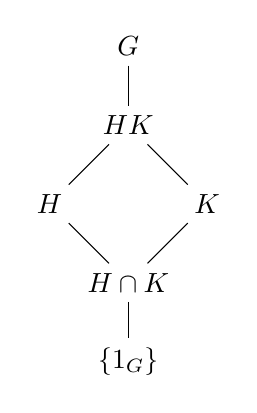
\begin{tikzpicture}
    \node (G) at (0,3) {\( G \)};
    \node (HK) at (0,2) {\( HK \)};
    \node (H) at (-1,1) {\( H \)};
    \node (K) at (1,1) {\( K \)};
    \node (HcapK) at (0,0) {\( H \cap K \)};
    \node (1G) at (0,-1) {\( \{1_G\} \)};
    
    \draw (G) -- (HK);
    \draw (HK) -- (H);
    \draw (HK) -- (K);
    \draw (H) -- (HcapK);
    \draw (K) -- (HcapK);
    \draw (HcapK) -- (1G);
\end{tikzpicture}
\end{center}

\begin{lemme}
        Si \( H \triangleleft G \) alors
\[
HK = \{ hk \mid h \in H, k \in K \} = \{ kh \mid k \in K, h \in H \}.
\]
    \end{lemme}

\begin{proof}
    Soient \( h \in H \) et \( k \in K \). Alors  
\[
kh = \underbrace{(khk^{-1})}_{\in H} k \quad \text{et} \quad hk = k \underbrace{(k^{-1}hk)}_{\in H}
\]
car \( H \triangleleft G \). On en déduit la deuxième égalité dans (4.1).  
De plus, on a que \( HK = \{ k_1h_1 \dots k_nh_n \mid n \geq 1, h_i \in H, k_i \in K \} \) et  
\[
k_1h_1k_2h_2 = k_1 \underbrace{k_2 (k_2^{-1}h_1k_2)}_{\in H} h_2
\]
car \( H \triangleleft G \). Par induction, \( HK = \{ kh \mid k \in K, h \in H \} \). \(\square\)

\end{proof}

 \begin{proposition}
        Soient \( H \triangleleft G \) et \( K < G \). Le morphisme \( K \to G/H \),  
\( k \mapsto kH \) induit un isomorphisme
\[
K / (K \cap H) \simeq HK / H.
\]
    \end{proposition}

Noter que \( H \triangleleft G \) implique \( H \triangleleft HK \) et \( K \cap H \triangleleft K \). 
\begin{proof}
    Soit \( f : K \to G/H \), \( k \mapsto kH \) la restriction à \( K \) de \( \pi_H : G \twoheadrightarrow G/H \).  
Alors 
\[
\ker(f) = \{ k \in K \mid kH = H \} = K \cap H.
\]
Comme \( H \triangleleft G \), on a  
\[
HK = \{ kh \mid k \in K, h \in H \},
\]
d'où  
\[
\text{im}(f) = \{ kH \mid k \in K \} = \{ khH \mid k \in K, h \in H \} = HK/H.
\]
Par factorisation on obtient un isomorphisme \( K / (K \cap H) \simeq HK / H \). \(\square\)
\end{proof}

  \begin{corollaire}
        Si \( H \triangleleft G \) et \( K < G \) alors
\[
|HK| = \frac{|H| |K|}{|H \cap K|}.
\]
    \end{corollaire}

\begin{proposition}
        Soient \( H, K < G \) tels que \( H \cap K = \{ 1_G \} \) et \( hk = kh \) pour tous \( h \in H, k \in K \). Alors on a un isomorphisme
\[
\left\{
\begin{array}{ccc}
H \times K & \simeq & HK \\
(h, k) & \mapsto & hk.
\end{array}
\right.
\]
\end{proposition}

\section{Groupes de permutations}

\begin{notation}
    On notera l'ensemble $\{1,2,\cdots,n\}$ par $[[a,b]]$. On notera l’ensemble de bijection de $[[1,n]]$ dans lui même i.e $\Sg([[1,n]])$ par
    \[
    \Sg_n
    \]
\end{notation}

\begin{remarque}
    Par des éléments élémentaires de combinatoire on peut se convaincre que $|\mathfrak{S}_n|=n!$
\end{remarque}

Soit $\sigma \in \Sg_n$ On notera la bijection \[\sigma:[[1,n]]\to [[1,n]], \: 1\mapsto \sigma(1), \: 2\mapsto \sigma(2), ..., n\mapsto \sigma(n)\]
    Par 
   \[
  \sigma = \begin{pmatrix}
      
 
    1 & 2 & 3 & \cdots & n-1 & n \\
    \sigma(1) & \sigma(2) & \sigma(3) & \cdots &  \sigma(n-1)  & \sigma(n)
  \end{pmatrix}
\]
De plus $\forall \sigma, \tau \in \Sg_n$, on notera,\\
\[
\sigma\circ\tau = \sigma \tau
\]
\begin{proposition}
        On a que $(\Sg_n, \circ)$ forme un groupe. On appelle ce groupe, le groupe symétrique d'indice n (ou groupe de permutations)
    \end{proposition}

\begin{proof}
    Montrons l'associativité,
    $\forall\nu,\sigma ,\tau \in \Sg_n, \: \forall i\in [[1,n]]$ on a 
    \[
    (\nu(\sigma \tau))(i)=\nu(\sigma(\tau(i))=((\nu\sigma)\tau)(i)
    \]
    L'existence du neutre
    \[
    \forall \nu \in \Sg_n \quad id\cdot\nu =\nu \cdot id = \nu 
    \]
    De plus, On a montrer que si une fonction est bijective sont inverse l'est aussi d'où
    \[
    \forall \nu \in \Sg _n, \exists\: \tau \in \Sg _n, \quad \nu \tau =\tau \nu = id  
    \]
\end{proof}

\begin{remarque}
    $\forall \nu \in \Sg_n,$ on a que $\nu^{-1}$ est obtenu en inversant les deux ligne de $\nu$
\end{remarque}

\begin{exemple}
    On prend $\nu \in \Sg_3$ tel que $\nu: [[1,3]]\to [[1,3]], \: 1\mapsto 2, \: 2\mapsto3, \: 3\mapsto 1$ c'est à dire ,
\[
\nu = \begin{pmatrix}
    1 &2&3\\ 2 &3 & 1
\end{pmatrix}
\]
On a $\nu^{-1}: [[1,n]]\to [[1,n]], \: 1\mapsto 3, \: 2 \mapsto 1, \: 3\mapsto 1$. c'est à dire,
\[
\nu^{-1}=\begin{pmatrix}
    1&2&3\\3&1&2
\end{pmatrix}
\]
On a bien 
\[
\nu^{-1}\nu= \begin{pmatrix}
    1&2&3\\3&1&2
\end{pmatrix}\cdot\begin{pmatrix}
    1&2&3\\ 2&3&1
\end{pmatrix}=\begin{pmatrix}
    1&2&3\\1&2&3
\end{pmatrix}=id
\]
\end{exemple}
\begin{exemple}[\textbf{Étude du groupe $\Sg_3$}]
Commençons par exhiber tous les éléments du groupe. Voici les permutations du groupe $\Sg_3$.
\begin{align*}
    \nu_1&= \begin{pmatrix}
        1&2&3\\1&2&3
    \end{pmatrix}\\
    \nu_2&= \begin{pmatrix}
        1&2&3\\1&3&2
    \end{pmatrix}\\
    \nu_3&=\begin{pmatrix}
        1&2&3\\2&1&3
    \end{pmatrix}\\
    \nu_4&=\begin{pmatrix}
        1&2&3\\2&3&1
    \end{pmatrix}\\
    \nu_5&= \begin{pmatrix}
        1&2&3\\3&1&2
    \end{pmatrix}\\
    \nu_6&=\begin{pmatrix}
        1&2&3\\3&2&1
    \end{pmatrix}
\end{align*}
\end{exemple}

\begin{definition}
        Le support de $\sigma\in \Sg_n$\\
        \[
        \operatorname{supp}(\sigma)=\{k\in [[1,n]]\: |\: \sigma(k)\neq k\}
        \]
    \end{definition}

\begin{remarque}
    Noter que $\sigma(i) \neq i$ équivaut à $\sigma(\sigma(i)) \neq \sigma(i)$ puisque $\sigma$ est injective. On a donc
    \[
    i\in \operatorname{supp}(\sigma) \quad \Leftrightarrow \quad \sigma(i)\in \operatorname{supp}(\sigma)
    \]
\end{remarque}
\begin{remarque}
    Nous avons les propriétés suivantes:
    \begin{enumerate}
        \item $\operatorname{supp}(\sigma)=\operatorname{supp}(\sigma^{-1})$
        \item $\forall k \in \Z,\: \operatorname{supp}(\sigma^k)\subseteq\operatorname{supp}(\sigma)$
    \end{enumerate}
\end{remarque}

\begin{definition}
        Deux permutations $\mu,\sigma\in \Sg_n$ si l'une laisse invariants les nombres modifiés par l'autre. Ainsi,
    \[
    \mu(i)\neq i \Rightarrow \sigma(i)=i
    \]
    Auquel cas, on a aussi
    \[
    \sigma(i)\neq i \Rightarrow\mu(i)=i
    \]
    Autrement dit $\sigma$ et $\mu$ sont disjointes si et seulement si
    \[
    \operatorname{supp}(\sigma)\cap \operatorname{supp}(\mu)=\emptyset
    \]
    \end{definition}

    \begin{proposition}
        Deux permutations sont $\tau$  et $\sigma$ sont disjointes si et seulement si elles commutent, i.e
        \[
        \operatorname{supp}(\tau)\cap \operatorname{supp}(\sigma)=\emptyset \: \Rightarrow \:\tau \sigma=\sigma\tau
        \]
    \end{proposition}

\begin{proof}
C'est clair si $\sigma = \text{Id}$ ou $\tau = \text{Id}$. Supposons $\text{Supp}(\sigma)$ et $\text{Supp}(\tau)$ disjoints et non vides.  
Soit $i \in [[1, n]]$. Rappelons que $i \in \text{Supp}(\sigma)$ ssi $\sigma(i) \in \text{Supp}(\sigma)$ par 1.15. Trois cas se présentent.

\begin{itemize}
    \item Si $i \notin \text{Supp}(\sigma) \sqcup \text{Supp}(\tau)$ alors $(\sigma \tau)(i) = \sigma(i) = i$ et $(\tau \sigma)(i) = \tau(i) = i$.
    \item Si $i \in \text{Supp}(\sigma)$ alors $i \notin \text{Supp}(\tau)$ et $\sigma(i) \notin \text{Supp}(\tau)$, d'où $(\sigma \tau)(i) = \sigma(i)$ et $(\tau \sigma)(i) = \sigma(i)$.
    \item Si $i \in \text{Supp}(\tau)$ alors $i \notin \text{Supp}(\sigma)$ et $\tau(i) \notin \text{Supp}(\sigma)$, d'où $(\sigma \tau)(i) = \tau(i)$ et $(\tau \sigma)(i) = \tau(i)$.
\end{itemize}

Par conséquent $\sigma \tau = \tau \sigma$.
\end{proof}
\begin{remarque}
    Si $\sigma\tau=\tau\sigma$ alors, $(\sigma\tau)^k=\sigma^k\tau^k$ pour tout $k\in \Z$
\end{remarque}
Soit $\sigma \in S_n$. On définit une relation binaire sur $[[1, n]]$ par :

\[
i \sim_{\sigma} j \iff \exists k \in \mathbb{Z} \mid \sigma^k(i) = j.
\]

C'est une \textit{relation d'équivalence} (réflexive, symétrique, transitive) :

\[
\begin{aligned}
    &i \sim_{\sigma} i \quad &&\text{car } \sigma^0(i) = \text{Id}(i) = i \\ 
    &i \sim_{\sigma} j \iff j \sim_{\sigma} i \quad &&\text{car } \sigma^k(i) = j \iff \sigma^{-k}(j) = i \\ 
    &(i \sim_{\sigma} j \wedge j \sim_{\sigma} r) \Rightarrow i \sim_{\sigma} r \quad &&\text{car } (\sigma^k(i) = j \wedge \sigma^\ell(j) = r) \Rightarrow \sigma^{\ell+k}(i) = \sigma^\ell(\sigma^k(i)) = \sigma^\ell(j) = r.
\end{aligned}
\]

La classe d’équivalence de $i \in  [[1, n]]$, appelée \textit{$\sigma$-orbite} de $i$, est

\[
\text{Orb}_{\sigma}(i) = \{\sigma^k(i) ; k \in \mathbb{Z} \}.
\]

La $\sigma$-orbite de $i$ décrit la trajectoire des itérés (avant ou arrière) de $\sigma$ en partant de $i$.

\begin{remarque}
    Les propriétés suivantes concernent le cardinal des orbites.

\begin{enumerate}
    \item $\# \text{Orb}_{\sigma}(i) = 1$ ssi $\text{Orb}_{\sigma}(i) = \{i\}$ ssi $\sigma(i) = i$ ssi $i \notin \text{Supp}(\sigma)$.
    \item Si $\text{ord}(\sigma) = d$ alors $\{\sigma^k(i) ; k \in \mathbb{Z} \} = \{\sigma^k(i) ; 0 \leq k < d\}$, d’où $\# \text{Orb}_{\sigma}(i) \leq d$.
    \item La partition de $[[1,n]]$ en orbites $(*)$ implique $\sum_{1 \leq m \leq r} \# \text{Orb}_{\sigma}(i_m) = n$.
\end{enumerate}
\end{remarque}

 \begin{proposition}
        Nous avons,
        \begin{enumerate}
            \item \textit{si} $\# \text{Orb}_{\sigma}(i) = s$ \textit{alors} $\text{Orb}_{\sigma}(i) = \{i, \sigma(i), \dots, \sigma^{s-1}(i)\}$~;
    \item $\sigma$ \textit{envoie} $\sigma^k(i)$ \textit{sur} $\sigma^{k+1}(i)$ \textit{si} $0 \leq k < s-1$, \textit{et} $\sigma^{s-1}(i)$ \textit{sur} $i$.
    \end{enumerate}
    \end{proposition}

\begin{definition}
        
            Considérons $t_1,t_2,\cdots,t_p\in [[1,n]]$,$p\geq 1,$ et les $n-p$ autres éléments $t_{p+1},\cdots,t_n \in [[1,n]]$. Le cycle associé à $t_1,\cdots,t_p$ est
            \[
            \begin{pmatrix}
                t_1 &t_2&\cdots&t_{p-1}&t_p&t_{p+1}&\cdots&t_n\\
                t_2&t_3&\cdots&t_p&t_1&t_{p+1}&\cdots& t_n          \end{pmatrix}
            \]
            Ainsi, cette permutation remplace $t_1,\cdots,t_{p-1}$ par l'élément suivant, $t_p$ par $t_1$ et laisse inchangés les autres éléments.
            On note ce cycle
            \[
            \begin{pmatrix}
                t_1&t_2&\cdots&t_{p-1}&t_p
            \end{pmatrix}
            \]
            on dit que $t_1,\cdots,t_p$ sont des éléments du cycle et que $p$ est sa longueur, on dit aussi que c'est un $p$-cycle.
            Autrement dit,
            Soit $2 \leq s \leq n$. Un cycle de longueur s dans $\Sg_n$ est une permutation de $[[1,n]]$
n’ayant qu’une seule orbite de cardinal s. Un cycle de longueur s est aussi appelé s-cycle.
    \end{definition}

\begin{remarque}
    L’écriture des cycles n’est pas unique, on peut faire tourner les ´éléments de
l’orbite en conservant l’ordre :
\[
\forall 1\leq t\leq s,\quad \begin{pmatrix}
    a_1&a_2&\cdots&a_s
\end{pmatrix}=\begin{pmatrix}
    a_t&a_{t+1}&\cdots&a_s&a_1&\cdots &a_{t-1}
\end{pmatrix}
\]
\end{remarque}

\begin{proposition}
    Toute permutation distincte de $id$ est un produit de cycles disjoints. Si on omet les cycle de longueur $1$, cette décomposition est unique à l'ordre des facteurs près.
\end{proposition}

\begin{proof}
Soit $\mu$ une permutation distinct de $id$. Fixons $i\in [[1,n]]$ et considérons l'orbite de $i$
\[
C_i=\{\mu^k(i)\: |\: k\in \Z\}
\]
son orbite est finie puisque $[[1,n]]$ est un ensemble fini. Ainsi il existe $p$ et $q$ des entiers positifs tels que
\[
\mu^p(i)=\mu^q(i)
\]
On peut supposer que \( p < q \). Dès lors, \( q - p \) est un entier positif tel que  
\[
\mu^{q - p}(i) = i.
\]
Soit \( m_i \), le plus petit entier positif ayant la propriété \( \mu^{m_i}(i) = i \).  
De cette définition, il résulte que  
\[
i, \mu(i), \dots, \mu^{m_i - 1}(i)
\]
sont distincts deux à deux. De plus,  
\[
C_i = \{ i, \mu(i), \dots, \mu^{m_i - 1}(i) \} = \{ \mu^k(i) \mid k \in \mathbb{Z} \}.
\]
En effet, si on effectue la division euclidienne de \( k \in \mathbb{Z} \) par \( m_i \), alors il existe \( q \in \mathbb{Z} \) tel que  
\[
k = q m_i + r \quad \text{avec } 0 \leq r < m_i.
\]
Or, puisque \( \mu^{m_i}(i) = i = \mu^{-m_i}(i) \), on a  
\[
\mu^k(i) = \mu^r(i) \quad \text{avec } 0 \leq r < m_i.
\]

de plus les orbites \( C_i \) forment une partition de \( [[1,n]] \).  


Choisissons à présent \( i_1, \dots, i_p \in [[1,n]] \) tels que \( C_{i_1}, \dots, C_{i_p} \) soient deux à deux disjoints et forment une partition de \( [[1,n]] \). Vu ce qui précède, on vérifie aisément que  
\[
\gamma_1 = ( i_1 \ \mu(i_1) \ \dots \ \mu^{m_{i_1} - 1}(i_1) )
\]
\[
\vdots
\]
\[
\gamma_p = ( i_p \ \mu(i_p) \ \dots \ \mu^{m_{i_p} - 1}(i_p) )
\]
sont des cycles disjoints tels que \( \mu = \gamma_1 \dots \gamma_p \).  
Comme les cycles de longueur 1 sont égaux à l’identité, on peut les omettre sans changer la valeur du produit.

Pour conclure, il nous faut encore montrer l’unicité de la décomposition.  
Supposons que \( \mu = \gamma_1' \dots \gamma_q' \) où \( \gamma_1', \dots, \gamma_q' \) sont des cycles disjoints de longueur au moins égale à 2.  
Soient \( k \in \{1, \dots, q\} \) et \( x \) un élément du cycle \( \gamma_k' \).  
Puisque \( \gamma_k' \) est un cycle, l’ensemble \( \{ \mu^i(x) \mid i \in \mathbb{Z} \} \) est exactement l’ensemble des éléments apparaissant dans \( \gamma_k' \)  
et coïncide avec un des \( C_{i_1}, \dots, C_{i_p} \).  
Réciproquement, pour tout \( j \in \{1, \dots, p\} \), \( C_{i_j} \) coïncide avec l’ensemble des éléments d’un des cycles \( \gamma_k' \).
\end{proof}

\begin{lemme}
        \textit{Si $\gamma$ est un $s$-cycle alors $\operatorname{ord}(\gamma) = s$.}

\medskip

Autrement dit, l’ordre d’un cycle est sa longueur.

    \end{lemme}

\begin{proof}
    Soit $\gamma = (a_1\ a_2\ \dots\ a_s) \in S_n$ un $s$-cycle. Pour tout $1 \leq k \leq s$, on a :

\[
\gamma(a_k) = a_{k+1}, \quad \gamma^2(a_k) = a_{k+2}, \quad \dots, \quad \gamma^{s-k}(a_k) = a_{k+s-k} = a_s.
\]

Ainsi, en continuant :

\[
\gamma^{s-k+1}(a_k) = a_1, \quad \gamma^{s-k+2}(a_k) = a_2, \quad \dots, \quad \gamma^{s-1}(a_k) = a_{k-1}, \quad \gamma^s(a_k) = a_k.
\]

Par ailleurs, pour tout $i \notin \operatorname{Supp}(\gamma)$, on a $\gamma^m(i) = i$ pour tout $m \geq 1$. Les $s$ éléments $a_1, \dots, a_s$ étant distincts, $s$ est le plus petit entier $\geq 1$ tel que $\gamma^s = \text{Id}$.

\medskip

Donc $\operatorname{ord}(\gamma) = s$.
\end{proof}

\begin{remarque}
     \textit{Soit $\sigma = \gamma_1 \dots \gamma_r$ la décomposition de $\sigma$ en cycles disjoints. Les $\gamma_i$ commutent entre eux, donc}  

\[
\forall k \in \mathbb{Z}, \quad \sigma^k = (\gamma_1 \dots \gamma_r)^k = \gamma_1^k \dots \gamma_r^k.
\]
\end{remarque}

 \begin{proposition}
        Soit $\sigma\in \Sg_n$, $\sigma \neq id$ et $\sigma= \gamma_1\gamma_2\cdots\gamma_r$ sa décomposition en cycles disjoints de longueur $s_1,s_2,...,s_r$ alors,
        \[
        \operatorname{ord}(\sigma)=\operatorname{ppcm}(s_1,s_2,...,s_r)
        \]
\end{proposition}

\begin{proof}
    Par le Lemme, l'ordre d'un cycle $\gamma_i$ est égal à sa longueur $s_i$, c'est-à-dire que $\gamma_i^{s_i} = \text{Id}$ et que $s_i$ est le plus petit entier vérifiant cette propriété.  

Par la Remarque, puisque les cycles $\gamma_i$ sont disjoints, ils commutent, donc pour tout entier $k \in \mathbb{Z}$ :
\[
\sigma^k = (\gamma_1 \dots \gamma_r)^k = \gamma_1^k \dots \gamma_r^k.
\]
Ainsi, pour que $\sigma^k = \text{Id}$, il faut et il suffit que $\gamma_i^k = \text{Id}$ pour tout $i$, c'est-à-dire que $k$ soit un multiple de chaque $s_i$.  

L'ordre de $\sigma$ est alors le plus petit entier $k$ satisfaisant cette condition, soit le **plus petit commun multiple** des longueurs des cycles :
\[
\operatorname{ord}(\sigma) = \operatorname{ppcm}(s_1, \dots, s_r).
\]
\end{proof}

\begin{definition}
    Une transposition est un $2$-cycle. Une transposition est une permutation qui permute deux éléments distincts et laisse les autres éléments inchangés.
\end{definition}

\begin{remarque}
    On a que le nombre de transposition dans le groupe $\Sg_n$ est $\begin{pmatrix}
        n\\2
    \end{pmatrix}=\frac{n(n-1)}{2}$
\end{remarque}

\begin{proposition}
        Tout $p$-cycle est un produit de $p-1$ transpositions.
    \end{proposition}

\begin{proof}

Considérons un cycle de longueur \( p \), noté :
\[
\gamma = (a_1 \ a_2 \ \dots \ a_p).
\]
Par définition, ce cycle envoie \( a_1 \) sur \( a_2 \), \( a_2 \) sur \( a_3 \), et ainsi de suite, jusqu’à \( a_p \) qui est envoyé sur \( a_1 \).

Nous allons montrer que ce cycle peut s’écrire comme un produit de \( p-1 \) transpositions. Plus précisément, nous affirmons que :
\[
(a_1 \ a_2 \ \dots \ a_p) = (a_1 \ a_p)(a_1 \ a_{p-1}) \dots (a_1 \ a_2).
\]
Montrons par récurrence que ce produit de transpositions donne bien le cycle initial.

\textbf{Base de récurrence :}  
Pour \( p = 2 \), un 2-cycle est simplement une transposition, ce qui est trivial.

\textbf{Hérédité :}  
Supposons que pour un cycle de longueur \( p-1 \), on puisse l’écrire comme un produit de \( p-2 \) transpositions. Montrons que cela reste vrai pour un cycle de longueur \( p \).

Considérons la permutation \(\sigma = (a_1 \ a_2 \ \dots \ a_p)\). Décomposons son action sur les éléments :

- La transposition \( (a_1 \ a_p) \) échange \( a_1 \) et \( a_p \).
- La transposition \( (a_1 \ a_{p-1}) \) place \( a_{p-1} \) à la position de \( a_1 \), et ainsi de suite.
- À la fin, en appliquant successivement les transpositions \( (a_1 \ a_p), (a_1 \ a_{p-1}), \dots, (a_1 \ a_2) \), on obtient exactement le cycle \( (a_1 \ a_2 \dots a_p) \).

Ainsi, par récurrence, tout cycle de longueur \( p \) est un produit de \( p-1 \) transpositions.

\end{proof}

 \begin{corollaire}
        Toute permutation est un produit de transposition.
    \end{corollaire}

\begin{definition}
        Soit $\sigma$ une permutation de $[[1,n]]$ et soit $i,j\in [[1,n]]$.\\
        La paire $\{i,j\}$ est une inversion de $\sigma$ si
        \[
        i<j \quad \text{et} \quad \sigma(i)>\sigma(j)
        \]
        ou
        \[
        i>j \quad \text{et}\quad \sigma(i)<\sigma()
        \]
    \end{definition}

 \begin{proposition}
        Soient $\mu,\nu \in \Sg_n$. On a
        \[
        \operatorname{sign}(\mu\nu)=\operatorname{sign}(\mu)\operatorname{sign}(\nu)
        \]
\end{proposition}

\begin{proof}
    
Soient \(\mu, \nu \in \mathfrak{S}_n\). Le nombre d’inversions de la permutation composée \(\mu\nu\) est donné par :

\[
\ell(\mu\nu) = \ell(\mu) + \ell(\nu) \mod 2.
\]

En effet, une inversion dans \(\mu\nu\) provient soit d’une inversion déjà présente dans \(\mu\), soit d’une inversion due à \(\nu\), et chaque inversion contribue additivement au nombre total d’inversions modulo 2.

En prenant l'exponentielle \( (-1) \) de chaque côté, on obtient :

\[
(-1)^{\ell(\mu\nu)} = (-1)^{\ell(\mu) + \ell(\nu)} = (-1)^{\ell(\mu)} (-1)^{\ell(\nu)}.
\]

Or, par définition du signe d’une permutation,

\[
\operatorname{sign}(\mu\nu) = (-1)^{\ell(\mu\nu)}
\]
\end{proof}

\begin{corollaire}
        Dans une décomposition d'une permutation en transpositions. Le nombre de facteurs est pair (resp. impair) si la permuation est pair(resp. impair)
    \end{corollaire}

\begin{corollaire}
        Tout cycle de longueur paire (resp. impaire) est une permutation impair (resp. paire). De plus, la parité d'une permutation est la parité du nombre de ses cycles de longueur paire.
    \end{corollaire}

\begin{proposition}
        le nombre de permutation paire de $\Sg_n$ est égale au nombre de permutation impaires de $\Sg_n$ et vaut $n!/2$.
        On note l'ensemble des permutations paires $\mathcal{A}_n$
\end{proposition}

\begin{proof}
 Soient \(\mu_1, \dots, \mu_k\) les permutations paires de \(\{1, \dots, n\}\).  
Puisque \(n > 1\), il existe au moins une permutation impaire \(\tau\). Au vu de la proposition IV.4.4, les permutations \(\tau \mu_1, \dots, \tau \mu_k\) sont impaires. De plus, ces dernières permutations sont deux à deux distinctes. En effet, supposons que \(\tau \mu_i = \tau \mu_j\) avec \(i \neq j\). En multipliant à gauche par \(\tau^{-1}\), on trouve \(\mu_i = \mu_j\).  

Enfin, il n’y a pas d’autre permutation impaire que \(\tau \mu_1, \dots, \tau \mu_k\). En effet, supposons que \(\nu\) soit une permutation impaire distincte de \(\tau \mu_i\) pour tout \(i \in \{1, \dots, k\}\). Dès lors, \(\tau^{-1} \nu\) est une permutation paire. Donc il existe \(j \in \{1, \dots, k\}\) tel que \(\tau^{-1} \nu = \mu_j\) et  
\[
\nu = \tau \tau^{-1} \nu = \tau \mu_j.
\]

\end{proof}

\begin{proposition}
        Le groupe $\mathcal{A}_n$ est engendré par les $3$-cycles
\end{proposition}

\begin{proof}
    Tout ´élément de $\mathcal{A_n}$ ´étant un produit d’un nombre pair de transpositions, il suffit de
vérifier que tout produit de deux transpositions distinctes est aussi un produit de 3-cycles.
Soient $(i j),(r s) \in \Sg_n$ des transpositions distinctes. Si leurs supports ne sont pas disjoints,
alors ils ont un élément commun, disons $j = r$ ; dans ce cas
$(i j)(j s) = (i j s)$.
Si leurs supports sont disjoints, alors on vérifie aisément que
$(i j)(r s) = (i j r)(j r s)$.
\end{proof}

 \begin{theoreme}
        Pour $n\geq 5$, le groupe $\mathcal{A}_n$ est simple.
    \end{theoreme}

\section{Action de groupe}
\begin{definition}
    Soient $(G,*)$ un groupe et $X$ un ensemble. On dit que $\fonction{\cdot}{G\times X\to X}{(g,x)\mapsto g\cdot x}$ est une action de $G$ sur $X$ si 
    \begin{itemize}
        \item $\forall g,h\in G, \forall x\in X,\ g\cdot(h\cdot x)=(g*h)\cdot x$
        \item $\forall x\in X,\ 1_G\cdot x = x$
    \end{itemize}
\end{definition}

\begin{definition}
    On dit que $G$ agit sur $X$ via $\rho$ si 
    \begin{equation*}
        \fonction{\rho}{G\to\Sg(G)}{g\mapsto \rho_g}
    \end{equation*}
    est un morphisme
\end{definition}

\begin{proposition}
Les définitions d'action de groupe par morphisme et par opération sont équivalentes, \textit{i.e.} à chaque action de groupe $\cdot$, on peut associer un morphisme $\rho$ définissant une action de $G$ sur $X$
\end{proposition}

\begin{proof}
    Soit $(G,*)$ un groupe. Soit $X$ un ensemble
    Soit $\cdot$ une action de $G$ sur $X$. Montrons que $\forall g\in G$ l'application $$\fonction{\rho_g}{X\to X}{x\mapsto g\cdot x}$$ est bijective. Soit $x\in X$. Commençons par montrer que $\forall g,h\in G, \rho_g\circ\rho_h=\rho_{g*h}$. Soit $x\in X$. On a $\rho_g\circ\rho_h(x)=g\cdot(h\cdot x)=(g*h)\cdot x = \rho_{g*h}(x)$. Il vient donc $\rho_g\circ\rho_{g^{-1}} = \rho_{1_G} = \rho_{g^{-1}}\circ \rho_g = \operatorname{Id}_X$ car $\forall x, 1_G\cdot x = x$. Donc $\rho_g$ admet un inverse pour $\circ$, \textit{i.e.} $\rho_g$ est bijectif. On peut donc définir l'application $$\fonction{\rho}{G\to\Sg(X)}{g\mapsto\rho_g}$$ et on a montré ci-dessus que $\rho$ est un morphisme de groupe.\\
    Soit $$\fonction{\rho}{G\to\Sg(G)}{g\mapsto\rho_g}$$ un morphisme de groupe. Montrons que $$\fonction{\cdot\ }{G\times X\to X}{(g,x)\mapsto \rho_g(x)}$$ est une action de groupe. Soient $h,g\in G, x\in X$. On a $g\cdot(h\cdot x)=\rho_g\circ\rho_h(x)=\rho_{g*h}(x) = (g*h)\cdot x$ car $\rho$ est un morphisme. De plus, on a $\rho_{1_G} = \operatorname{Id}_X$ car $\rho$ est un morphisme, d'où $ 1_G\cdot x = \rho_{1_G}(x)=x$.\\
    On doit encore montrer que l'application qui envoie une certaine action $\cdot$ sur $\rho^\cdot$ est l'inverse de celle envoyant un morphisme $\rho:G\to\Sg(X)$ sur une action $\cdot_\rho$; on ne le fera pas ici car c'est évident et cela demande d'introduire de lourdes notations.
\end{proof}

\begin{definition}
    Avec une action de groupe, on peut définir les ensembles suivants
    \begin{itemize}
    \item $\stab_x:=\{g\in G\mid g\cdot x = x\}$
    \item $\orb_X:=\{g\cdot x\mid g\in G\}$
    \end{itemize}
\end{definition}

\begin{proposition}
    $\forall x\in X,\ \stab_x$ est un sous-groupe de $G$.
\end{proposition}

\begin{proof}
    On a bien $1\in \stab_x$ par définition. De plus, avec $h,g\in \stab_x$, on a $(h*g)\cdot x = h\cdot(g\cdot x) = h\cdot x = x$, d'où $h*g\in\stab_x$. Donc $\stab_x<G$
\end{proof}

\begin{proposition}
    $X=\bigcup_{x\in X}\orb_x$ et $\forall x_1,x_2\in X,\ \orb_{x_1}\cap\orb_{x_2} = \varnothing$ ou $\orb_{x_1}=\orb_{x_2}$
\end{proposition}

\begin{proof}
    Considérons $\sim$ la relation binaire sur $X$ définie par 
\end{proof}

\begin{notation}
    Au cours de cette section, on sous-entendra que $G$ est un groupe, $X$ un ensemble non vide, $\cdot$ une action de $G$ sur $X$ et $\rho:G\to\Sg(G)$ le morphisme associé à $X$. 
\end{notation}

\begin{proposition}
    \begin{equation*}\fonction{\psi}{G/\stab_x\to\orb_x}{g\stab_x\mapsto g\cdot x}
    \end{equation*}
    est bijective.
\end{proposition}

\begin{proof}
\end{proof}

\section{Théorème de Syllow}

\begin{definition}
    Soient $G$ un groupe fini et $p$ un nombre premier divisant $|G|$. On écrit $|G|=p^\alpha m$, avec $p$ et $m$ premiers entre entre eux et $\alpha \geq 1$. Un $p$-sous-groupe de Syllow ou plus simplement un $p$-Syllow de $G$ est un sous-groupe de $G$ d'ordre $p^\alpha$
\end{definition}

\begin{proposition}
        Soient $G$ un groupe fini, $p$ un nombre premier divisant $|G|$ et $S$ un $p$-Syllow de $G$. Si $H$ est un sous-groupe de $G$, il existe $g\in G$ tel que $gSg^{-1}\cap H$ soit un $p$-Syllow de $H$.
\end{proposition}

\begin{proof}
    Le groupe \( G \) agit sur \( G/S \) par multiplication à gauche et cette action induit une action de \( H \) sur \( G/S \). Soit \( gS \in G/S \) une classe à gauche. On vérifie que, pour l’action de \( G \),
    \[
    \operatorname{Stab}_G(gS) = gSg^{-1}.
    \]
    
    En effet,
    \[
    hgS = gS \Longleftrightarrow g^{-1}hgS = S
    \Longleftrightarrow g^{-1}hg \in S
    \Longleftrightarrow h \in gSg^{-1}.
    \]
    
    Pour l’action de \( H \) induite par celle de \( G \), on a
    \[
    \operatorname{Stab}_H(gS) = gSg^{-1} \cap H.
    \]
    On va montrer que l’un des stabilisateurs \( \operatorname{Stab}_H(gS) \) est un \( p \)-Sylow de \( H \). Ces stabilisateurs sont des sous-groupes du \( p \)-groupe \( gSg^{-1} \), donc ce sont encore des \( p \)-groupes. Si l’indice de l’un de ces sous-groupes n’est pas multiple de \( p \), c’est forcément un \( p \)-Sylow de \( H \). D’autre part, puisque \( S \) est un \( p \)-Sylow de \( G \), le cardinal du quotient \( G/S \) n’est pas multiple de \( p \), et comme on a
    \[
    |G/S| = \sum_{i} |O_i|,
    \]
    où on somme sur toutes les orbites \( O_i \) distinctes sous l’action de \( H \). Il existe \( i_0 \) tel que \( |O_{i_0}| \) ne soit pas multiple de \( p \). Soit \( g \) vérifiant \( gS \in O_{i_0} \) ; le cardinal 
    \[
    |O_{i_0}| = |H / \operatorname{Stab}_H(gS)|
    \]
    est premier à \( p \), et \( \operatorname{Stab}_H(gS) \) est un \( p \)-Sylow de \( H \).
\end{proof}

\begin{remarque}
    On a 
    \[
    |GL_n(\mathbb{F}_p)|=(p^n-1)(p^n-p)\cdots(p-p^{n-1})
    \]
    En effet, il y a autant d'élément dans $GL_n(\mathbb{F}_p)$ que dans $\mathbb{F}_p^n$. Pour construire une base, on commence par choisir n'importe quel vecteur non nul de $GL_n(\mathbb{F}_p)$ comme l'image de $e_1$, puis on choisit n'importe quel vecteur qui ne lui est pas colinéaire, et ainsi de suite. En regroupant les puissances de $p$, on obtient
    \[
    |GL_n(\mathbb{F}_p)|=p^{n(n-1)/2}(p^n-1)\cdots(p-1)
    \]
    Donc si on a $H$ un sous groupe de $GL_n(\mathbb{F}_p)$ tel que
    \[
    |H|=p^{n(n-1)/2}
    \]
    alors c'est $p$-Syllow.
\end{remarque}

\begin{theoreme}[Premier théorème de Syllow]
        Soient $G$ un groupe fini et $p$ un diviseur premier de $|G|$. Alors $G$ contient au moins un $p$-Syllow.
\end{theoreme}

\begin{proof}
     Soit \( G \) un groupe fini quelconque d’ordre \( n \), et soit \( p \) un nombre premier diviseur de \( n \). D’après la proposition 8.2, il suffit de montrer qu’il existe une application injective de \( G \) dans un groupe admettant un \( p \)-Sylow. Le théorème de Cayley montre déjà que \( G \) est isomorphe à un sous-groupe de \( \mathfrak{S}_n \). Mais on peut construire un morphisme injectif de \( \mathfrak{S}_n \) dans \( GL_n(\mathbb{F}_p) \) : à une permutation \( \sigma \), on associe l’endomorphisme \( u_{\sigma} \) défini sur la base canonique par
    \[
    u_{\sigma}(e_i) = e_{\sigma(i)}, \quad 1 \leq i \leq n.
    \]
    L’application linéaire \( u_{\sigma} \) est inversible car \( \sigma \) est bijective, et on vérifie aisément que l’application \( \sigma \mapsto u_{\sigma} \) est un morphisme injectif. Or l’exemple 8.1 montre que \( GL_n(\mathbb{F}_p) \) admet un \( p \)-Sylow, ce qui clôt la preuve.
\end{proof}
\section{Groupe diédral}

\begin{tcolorbox}[colback=red, colframe=red]
\begin{center}
    En chantier
\end{center}
\end{tcolorbox}


\section{Groupes libres}

\begin{tcolorbox}[colback=red, colframe=red]
\begin{center}
    En chantier
\end{center}
\end{tcolorbox}

\begin{definition}
    A subset $X$ of a group $G$ is called  a \textbf{free set of generetors for G}, if every $g\in G\setminus \{e\}$ can be expressed in a unique way as a product 
    \begin{equation}\label{uniqueness}
        g=x_{1}^{n_1}x_{2}^{n_2}\dotsc x_{k}^{n_k}
    \end{equation}
    of finite length, where the $x_i$ lie in $X$, $x_i$ is never equal to $x_{i+1}$, and each $n_i$ is a non-zero integer. 
    We call the set of generetors free because by the uniqueness of \ref{uniqueness} there can be no relations between its elements.
    if $G$  has a free set of generetors then it is a \textbf{free group}.
\end{definition}

\begin{definition}
    Given a nonempty set $X$  we can construct a group which has $X$ as free set generators as follows.
    Define a \textbf{word} in the alphabet $X$ to be a finite product
    \begin{equation*}
        x_1^{m_1}x_2^{m_2}\dotsc x_s^{m_s}
    \end{equation*}
    in each $x_i$ belongs to $X$ and the $m_i$ are all integers, and say that the word is reduced if $x_i$ is never equal to $x_{i+1}$ and all the $m$ are non-zero. Each word can be simplified to a reduced word
    by collecting up powers when adjacent elements are equal, and omitting zeroth powers, continuing  this
    process serveral times if necessary.
\end{definition}

\begin{exemple}
    Take $X=\{x,y,z\}$ and consider the word
    \begin{equation*}
        w=x^{-3}x^2y^5y^{-5}x^7z^2z^{-2}x^{-1}xzy^2x^{-1}
    \end{equation*}
    Then 
    \begin{align*}
        w&=x^{-1}y^0x^7z^0x^0zy^2x^{-1}\\
        &= x^{-1}x^7zy^2x^{-1}\\
        &= x^6zy^2x^{-1}\\
    \end{align*}
    which is now reduced. Notice that the elements of $X$ do not commute with one another. It may be possible to carry out the actual process of reduction in more than one way, for exemple
    \begin{align*}
         w&=(x^{-3}x^2y^5y^{-5}x^7z^2)(z^{-2}x^{-1}xzy^2x^{-1})\\
         &=(x^{-1}y^0x^7z^2)(z^{-2}x^0zy^2x^{-1})\\
         &=(x^6z^2)(z^{-2}zy^2x^{-1})\\
         &=x^6z^2z^{-1}y^2x^{-1}\\
         &=x^6zy^2x^{-1}
    \end{align*}
\end{exemple}
 However, the end result is always the same, as we shall verify in \ref{reducedword}, and each word $w$ leads to a unique reduced word $\overline{w}$. Reducing the word $x_1^0$ gives a word with no symbols, which we refer to as the empty word. We can multiply words together simply by writing one after the other. If we do this with two reduced word $w_1$ and $w_2$, then $w_1w_2$ may not be reduced because the final symbol of $w_1$ may be the same as the firste symbol of $w_2$. But $w_1w_2$ simplifies to a reduced word $\overline{w_1w_2}$, and the set of all reduced words forms a group if we use $\overline{w_1w_2}$ as product. Associativity holds because $\overline{(\overline{w_1w_2})w_2}$ and $\overline{w_1(\overline{w_2w_3})}$ result from two different reductions of a word $w_1w_2w_3$, and are therefore both equal to the reduced word $\overline{w_1w_2w_3}$. The identity is the empty word, and the inverse of the reduced word
 \begin{equation*}
     x_1^{n_1}x_2^{n_2}\dotsc x_k^{n_k} \ \text{ is }\  x_1^{-n_1}x_2^{-n_2}\dotsc x_k^{-n_k}
 \end{equation*}
 which also reduced. This group of reduced words form the alphabet $X$ is called the \textbf{free group genereted by (the elements of) } $X$ and will be denoted by $F(X)$
 The preceding discussion depends crucially on the following result.

 \begin{theoreme}\label{reducedword}
     Each word can be simplified to only one reduced word.
 \end{theoreme}

 \begin{proof}
     We use an idea reminiscent of the proof of Cayley's theorem. For each $x\in X$ we produce a permutation $\varphi_x$ of the set of reduced words by the formula
     \begin{equation*}
         \varphi_x(w)=\overline{xw}
     \end{equation*}
     where $w$ is a reduced word. Clearly $\overline{xw}$ is well defined because $w$ is reduced. If
     \begin{equation*}
         u=x_1^{m_1}x_2^{m_2}\dotsc x_s^{m_s}
     \end{equation*}
     is an abritrary words we have the associated composite permutation
     \begin{equation*}
         \varphi_u=(\varphi_{x_1})^{m_1}(\varphi_{x_2})^{m_2}\dotsc(\varphi_{x_s})^{m_s}
     \end{equation*}
     Now the permutation of the reduced words form a group under composition of permutations and therefore if $u,w$ are words, and if $u$ reduces in some way to $w$, then $\varphi_u=\varphi_w$. Suppose the same words $u$ can be simplified in two different ways to give the reduced words $v$ and $w$. Then $\varphi_v=\varphi_{u}=\varphi_w$. But $\varphi_v$ sends the empty word to $v$, and $\varphi_w$ sends it to $w$, so we must have $v=w$
 \end{proof}

A free group which is genereted by a single element $x$ is infinite syclic, the only possible reduced words being the powers $x^n$. Xhen there are two ore more generetors, $F(X)$ is a non-abelian group  in which every element has infinite order. Notice that a bijection $\varphi$ from $X$ to $Y$ induces an isomorphism between $F(X)$ and $F(Y)$. The reduced word
\begin{equation*}
    x_1^{n_1}x_2^{n_2}\dotsc x_k^{n_k}
\end{equation*}
of $F(X)$ corresponds to the reduced word
\begin{equation*}
    \varphi(x_1)^{n_1}\varphi(x_2)^{n_2}\dotsc \varphi(x_k)^{n_k}
\end{equation*}
of $F(Y)$. Let $F_n$ stand for "the" group which is freely genereted by $n$ elements.

\begin{theoreme}
    Abelianising $F_n$ gives $\mathbb{Z}^n$.
\end{theoreme}

\begin{proof}
    Let $z_1,\dotsc,z_n$ be a free set of generators for $F_n$. The quotient group
    $F_n/[F_n,F_n]$ is abelian and is generated by the cosets $z_k[F_n,F_n], 1\leq k\leq n$. By collecting together powers of each generator, every element of this group can be written in precisely one way form
    \begin{equation*}
        z_1^{r_1}z_2^{r_2}\dotsc z_n^{r_n}[F_n,F_n]
    \end{equation*}
    the correspondence
    \begin{equation*}
        z_1^{r_1}z_2^{r_2}\dotsc z_n^{r_n}[F_n,F_n]\mapsto (r_1,r_2,\dotsc,r_n)
    \end{equation*}
    now provides an isomorphism between $F_n/[F_n,F_n]$ and $\mathbb{Z}^n$
\end{proof}

\begin{theoreme}
    If $F_m$ is isomorphic to $F_n$, then $m=n$.
\end{theoreme}

\begin{proof}
    For any two groups $G$, $H$ an isomorphism $\varphi:G\to H$ sends $[G,G]$ to $[H,H]$ because each commutator $xyx^{-1}y^{-1}$ in $G$ corresponds to the commutator $\varphi(x)\varphi(y)\varphi(x)^{-1}\varphi(y)^{-1}$ of $H$. So $\varphi$ induces an isomorphism from $G/[G,G]$ to $H/[H,H]$.Therefore, if $F_m$ is isomorphic to $F_n$ we have $\mathbb{Z}^m\simeq\mathbb{Z}^n$ and consequently $m=n$.
\end{proof}
Let $G$ be a group and supporse $X$ is a set of generator for $G$. There is a natural homomorphism $\pi$ from the free group $F(X)$ to $G$ which sends each reduced word
\begin{equation*}
    x_1^{n_1}x_2^{n_2}\dotsc x_k^{n_k}
\end{equation*}
onto the corresponding product of group elements in $G$. This homomorphism is surjective because $X$ generates $G$ and, if $N$ denotes its kernel, the first isomorphism theorem tells us that $F(X)/N$ is isomorphic to $G$. Therefore every group is a quotient of some free group. It is this result which will allow us to describe groups rigorously in terms of generators and relations. Let $R$ be a collection of words in $F(X)$ which together with all their conjugates generate $N$. That is to say, $N$ is the smallest normal group subgroup of $F(X)$ which contains $R$. These words determine precisely which words  in $F(X)$ become the identity when we pass from $F(X)$ to $G$ or, equivalently, which products of element of $G$ are the identity in $G$. We shall call $R$ a set of defining relations for $G$.

\begin{exemple}
    If $G=D_n$ and $X=\{r,s\}$, the words $r^n,s^2, (rs)^2$ form a set of defining relations for $G$. Let $M$ denotes the smallest normal subgroup of $F(X)$ which contains these three words and, as before, use $N$ for the kernel of the homomorphism $\pi : F(X)\to D_n$. We must show that $M=N$. Certainly  $r^n,s^2$ and $(rs)^2$ are all sent to the identity by $\pi$, so $M$ is contained in $N$ and by (un ref au troisieme theorem d'isomorphisme). We have a surjective homomorphism $F(X)/M\to F(X)/N$ whose kernel is $N/M$. In particular $\abs{F(X)/M}$ is at least $2n$. Now the cosets $rM,sM$ generate the quotient group $F(X)/M$ and they satisfy
    \begin{equation*}
     (rM)^n=M, \quad (sM)^2=M, \quad (rsM)^2=M
    \end{equation*}
        or equivalently
    \begin{equation}\label{D_n}
     (rM)^n=M, \quad (sM)^2=M, \quad srM=r^{n-1}sM
    \end{equation}
    be cause $r^n,s^2$ and $(rs)^2$ all belong to $M$. Using \ref{D_n} it is easy to show that the cosets
    \begin{equation*}
        M,rM,\dotsc,r^{n-1}M,sM,rsM,\dotsc,r^{n-1}sM
    \end{equation*}
    form a subgroup of $F(X)/M$. This subgroup contains $rM$ and $sM$ so it has to be the whole group $F(X)/M$. Therefore, $\abs{F(X)/M}$ is ar most $2n$. We conclude that $\abs{F(X)/M}=2n$ and $M=N$, as required.
\end{exemple}
Take a non-empty set $X$ and let $R$ be a collection of words in the alphabet $X$. The group determined by the set $X$ of generators and collection $R$ of defining relations is defined  to be the quotient group $F(X)/N$, where $N$ is the smallest normal subgroup of $F(X)/N$ which contains $R$. If $G$ as any group isomorphic to $F(X)/N$ the pair $X,R$ is called representation for $G$. In particular, if $X$ has a finite set with elements $x_1,\dotsc,x_s$ and if $R$ is a finite collection of words $w_1,\dotsc,w_t$ we say that $G$ is \textbf{finitely presented} and write
\begin{equation*}
    G\equiv\{x_1,\dotsc,x_s\mid w_1,\dots,w_t\}
\end{equation*}

\begin{exemple}
    \begin{enumerate}
        \item $\mathbb{Z}_n\equiv \{x\mid x^n\}$
        \item $D_n\equiv \{x,y\mid x^n,y^2,(xy)^2\}$
        \item For each integer $m\geq 2$ the presentation
        \begin{equation*}
            \{x,y\mid x^{2m},x^my^{-2},xyxy^{-1}\}
        \end{equation*}
        determines a group of order $4m$ called a dicyclic group
        \item $\mathbb{Z}\times\mathbb{Z}\equiv \{x,y\mid xyx^{-1}y^{-1}\}$
    \end{enumerate}
\end{exemple}
We can characterise free groups as follows
\begin{theoreme}
    Let $X$ be a subset of a group $G$. Then $X$ is a free set of generators for $G$ if and only if given an arbitrary group $H$, together with a fonction from $X$ to $H$, there is a unique extension of this function to a homomorphism from all of $G$ to $H$.
\end{theoreme}

\begin{proof}
    Suppose $X$ is a free set of generators for $G$. Then each element of $G\setminus\{e\}$ can be written in one and only one way as a reduced words in the alphabet $X$. Given a group $H$ and a function $f:X\to H$, the only way we can extend $f$ to a homomorphism from all of $G$ to $H$ is by sending each reduced word
    \begin{equation*}
        x_1^{n_1}x_2^{n_2}\dotsc x_k^{n_k}
    \end{equation*}
    to
    \begin{equation*}
        [f(x_1)]^{n_1}[f(x_2)]^{n_2}\dotsc [f(x_k)]^{n_k},
    \end{equation*}
    and the identity of $G$ to that of $H$
    For the controverse we assume that given a group $H$, together with a function from $X$ to $H$, we can always find a unique extension of this function to a homomorphisme from $G$ to $H$. As before, let $\pi:F(X)\to G$ be the homomorphism which sends eaxh reduced word to the same product thought of as an element of $G$. We shall show that $\pi$ is an isomorphism, when $X$ is certainly a free set of generators for $G$. Taking $H=F(X)$, the inclusion of $X$ into $F(X)$ extends to a homomorphism $\varphi:G\to F(X)$. Clearly, $\varphi\pi$ is the identity from $F(X)$ to $F(X)$ because $\varphi$ is the identity on $X$. Also, both $\pi\varphi:G\to G$ and the identity function from $G$ to $G$ are homomorphisms which extend the inclusion of $X$ in $G$ over all of $G$. By hypothesis there can only be one such extension, hence $\pi \varphi$ is the identity from $G$ to $G$. We conclude that $\pi$ is an isomorphism.
\end{proof}
